\documentclass{article}

\usepackage[utf8]{inputenc}
\usepackage[T1]{fontenc}
\usepackage[english]{babel}   %Engelsk først så norsk, så norsk blir prioritert
\usepackage{graphicx}
\usepackage{amsmath}        %For å kunne skrive matte
\usepackage{listings}       %For å kunne skrive inn kode med fin formatering
\usepackage{multicol}       %Importerer pakken for multikolonner til teksten
\usepackage[margin=2.54cm]{geometry}    %Definerer hva bredden til teksten er
\usepackage{wrapfig}    %Importerer pakken for å ha bildene i teksten
\usepackage[font = small]{caption}
\usepackage{textcomp}
\usepackage{mathrsfs}   %For å få fancy E til bildene

\usepackage{amssymb} %Fra Erlend for å bruke hakemerke?? Vet egt. ikke

%Definerer hyperlinker og dens farger
\usepackage{hyperref}
\hypersetup{
    colorlinks,
    citecolor=blue,
    filecolor=black,
    linkcolor=blue,
    urlcolor=blue
}

%-----------------------------------
\iffalse
%Definerer farger til kodeeksemplene i PDF-en
\usepackage{color}

\definecolor{codegreen}{rgb}{0,0.6,0}
\definecolor{codegray}{rgb}{0.5,0.5,0.5}
\definecolor{codepurple}{rgb}{0.58,0,0.82}
\definecolor{backcolour}{rgb}{0.95,0.95,0.92}

\lstdefinestyle{mystyle}{
    backgroundcolor=\color{backcolour},
    commentstyle=\color{codegreen},
    keywordstyle=\color{magenta},
    numberstyle=\tiny\color{codegray},
    stringstyle=\color{codepurple},
    basicstyle=\footnotesize,
    breakatwhitespace=false,
    breaklines=true,
    captionpos=b,
    keepspaces=true,
    numbers=left,
    numbersep=5pt,
    showspaces=false,
    showstringspaces=false,
    showtabs=false,
    tabsize=2
}

\lstset{style=mystyle}
\fi


%--------------------------------------

\setlength{\parindent}{0pt} %Ingen indent automatisk for nye linjer
%\setlength{\columnsep}{2mm} %Column separation - til multicolumn

%\setlength{\arrayrulewidth}{1mm}   %Hvilken tykkelse tabellene skal ha
\setlength{\tabcolsep}{2mm}     %Lengden mellom hver kolonne
\renewcommand{\arraystretch}{1.5}   %Hvor stor avstand det skal være mellom radene

\iffalse    %midlertidig endre bredden på teksten
If you want to change this temporarily, you can write:
\savegeometry{mydefaultgeometry}
\newgeometry{margin=3in}
And then later you can call:
\loadgeometry{mydefaultgeometry}
\fi

%for å fjerne overskriften "refrences" som kommer automatisk når man bruker bibtex
\usepackage{etoolbox}
\patchcmd{\thebibliography}{\section*{\refname}}{}{}{}

%lage exercises på norsk, slik at det står oppgave. også definere dette som en ny kommando
\newcounter{excount}
\newenvironment{exercise}[1][]{\addtocounter{excount}{1} \noindent {\bf Oppgave
\arabic{excount} \ \ #1}\hspace{2mm}}{\vspace{4mm}}


%----------------------

\usepackage{float}
%\restylefloat{table}

%----------------------

\usepackage{tikz}
\usetikzlibrary{patterns}

\usetikzlibrary{shapes.misc}
% From http://tex.stackexchange.com/questions/123760/draw-crosses-in-tikz
\tikzset{cross/.style={cross out, draw=black, fill=none, minimum size=2*(#1-\pgflinewidth), inner sep=0pt, outer sep=0pt}, cross/.default={3pt}}

\usetikzlibrary{decorations.markings}

%------------------

%dette brukes med \begin{python}
\usepackage{pythonhighlight}

\lstdefinestyle{mystyle}{
    numbers=left,
    numbersep=5pt,
}

\lstset{style=mystyle}


%-----------------------

%figurtekst under, tabelltekst over

%LEGGE TIL STJERNER VED SECTION FJERNER NUMMERERINGEN!!!!!!!!!!!!!!!!!!!!!!!!!!!!!!!!
%men da syntes ikke avsnittene i innholdsfortegnelsen!!!!!!!!!!!!!!!!!!!!!!!!!!!!!!!!

%------------------------------------------------------------------------------

\begin{document}

\addtocounter{page}{0}

\title{Project A20 \\
      \large FYS-MENA4111}
\date{\today \\
    \vspace{1mm}
    \large Week 44-48}

\author{Erlend Tiberg North \& Alexandra Jahr Kolstad}

\maketitle


%\newpage

%--------------- Her starter skrivingen ---------------------------------------

%\begin{multicols}{2}


%---------------------- Abstract -----------------------------------------
\vspace{1cm}


\begin{center}

{\Large\textbf{Abstract}} \label{sec:Abstract} \\

    \vspace{1mm}

    Quinizarin can function as an organic sensetizer in an upconversion system. In ALD the organic molecule can possibly be deposited in a matrix of lanthanide flouride, to increase the efficiency of the upconversion process in the material. To see how this efficiency can increase and what energy levels can be absorbed by the material, it is wise to investigate the electronic band structure of the molecule. This paper will look in to Quinizarin's own electronic properties, as well as, Quinizarin with lanthanides replacing one a Hydrogen atom, to emulate Quinizarin inside the structure in a simple way.

    \vspace{1cm}

\end{center}


\newpage

%-------------------- Table of contents -----------------------------------
\vspace{1cm}

\tableofcontents

\vspace{1cm}

%---------------------------------------------------------------------------------

\section{Introduction}  \label{sec:Introduction}

    Photons can be used for many things. However, not all photons are created equal. They come in many different energies, and not all energies are as simple to absorb. A way to increase the efficiency of photon-absorbing materials is by modifying it so that it can absorb photons with a low energy, collect that energy, and re-emit the photon with higher energy. This is known as up-conversion and has many uses. One use is to increase the efficiency of solar panels by allowing it to collect more of the sunlight, where the up-conversion system can be a thin-film on the top of the panel. A different use is to increase the energy to the point where the emitted photon can become ionizing and work as a bacteria or virus killer.\\

    Up-conversion is a phenomenon where incoming photons are re-emitted with a higher energy than they entered with. The photons excite electrons in a material, and by conduction of those electrons they can move to other atoms, where they are further excited. The electron ends up in a high energy state and de-excites releasing all the energy. However, the process can be very inefficient due to narrow energy bands in the material. A form of increasing this efficiency is by adding a material with a wide energy band to allow absorption of photons with more varied energy.\\

    This paper will focus on an organic compound known as Quinizarin. The compound is an organic dye and has a broad energy band. This means it can absorb a broad spectrum of photons energies. The excited electrons from this energy band can move to the actual up-conversion system and hereby increase the efficiency of the up-conversion. The planned up-conversion system will consist of Quinizarin as an organic sensitizer, Nd+3 and Yb+3 as electron migrators (transporting the electrons to the site of de-excitation), and Tm+3 as accumulator and activator (collecting excited electrons and up-converting them, and de-excitation site for said electrons). The system is planned to be inserted into a matrix of YbF3 or possibly YF3.\\

    Since Quinizarin is such an important piece of the system it is wise to know how it interacts with the other materials. This study will therefore investigate how Quinizarin's electronic band structure changes when the Hydrogen in the alcohol group is replaced with different atoms. In this case: Yb, Nd, Tm and Y. See figure~(\ref{fig:Quinizarin-X} for an illustration).\\

    \begin{figure}[H]
        \centering
        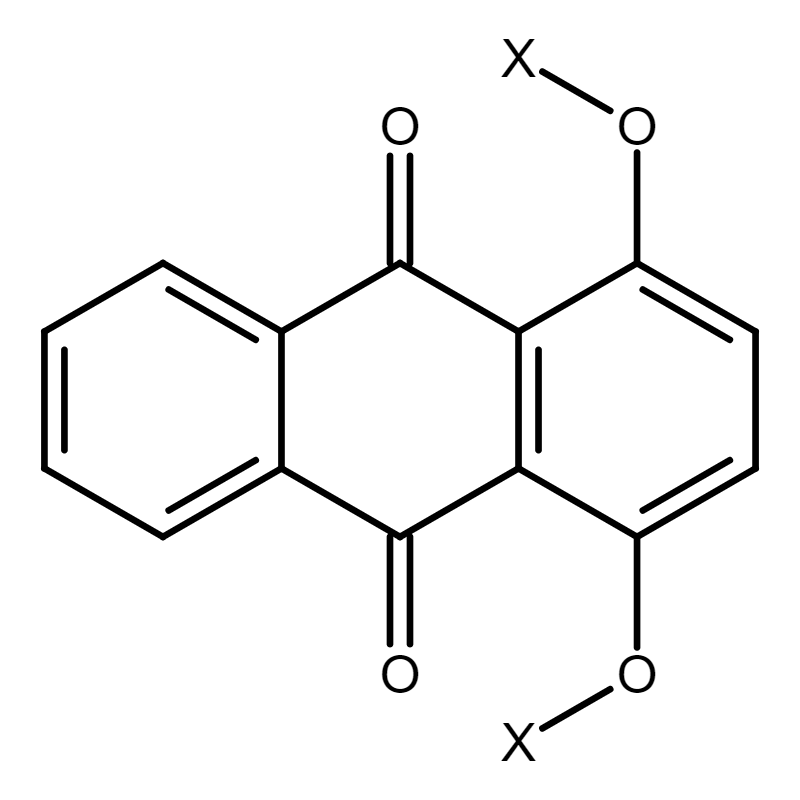
\includegraphics[width = 5cm]{../fig/quinizarin-x.png}
        \caption{Molecular structure of Quinizarin with H in -OH replaced with atom X. X can be H, Y, Yb, Nd or Tm. Structure drawn with online illustrator from \href{https://chem-space.com/search}{Chem-Space}.}
        \label{fig:Quinizarin-X}
    \end{figure}

\vspace{1cm}

\section{Method}    \label{sec:Method}

  The supercomputer Saga contains many different POSCAR-files for a wide range of structures. Unfortunately for us, Quinizarin was not included. Therefore we had to make our own POSCAR-file. This was done by drawing the structure in an organic compound structure program we found on the internet: \href{https://molview.org}{MolView}. This site lets the user draw organic structures with many varying features, and it also lets the user export the data as a \texttt{.mol}-file. A \texttt{.mol}-file has a similar structure with a POSCAR-file, which let us easily make the POSCAR-file for Quinizarin. \\

  The coordinates of the atoms in the \texttt{.mol}-file were put in a POSCAR file with Direct coordinates. We added a unit cell and, and opened it in VESTA. In order to make the plane-waves more stable for the calculations, we inserted a vacuum distance in each direction of 12 Å. \\

  To differentiate the two Hydrogen-atoms in the alcohol-groups from the other Hydrogen-atoms, we had to find their positions somehow. This was done in the program GeoGebra, by plotting each atom with their positions in 3D. We found that the Hydrogen-atoms were number 25 and 26 in POSCAR. In hindsight, we discovered that this would be easier to do in VESTA. \\

  In this project we will compare the basic Quinizarin with Quinizarin with both Yttrium (Y) and Ytterbium (Yb) substituted in the Hydrogen-positions described in the subsection above. Therefore we had to make in total three POSCAR-files for the three structures. This was done by opening POSCAR in Emacs and changing the two last atoms given in the file to the substitution-atoms. After that we ran in to issues with relaxing the structure, and so went to the ICSD database to find a decent distance between the new atoms and oxygen. We used approximately 2.3 Å in distance, and that worked well for relaxing the structure. \\


  \subsection{Convergence}  \label{sec:Convergence}

    Testing for convergence of energy and k-point is important to determine if the variables in INCAR or KPOINTS are good enough to be used for further calculations, mostly to ensure decent and applicable results. If the error is less than $1\cdot 10^{-3}$ the calculation can be considered converged. \\

    The testing of convergence is done by performing VASP calculations with different values of either energy-cutoff (ENCUT) or k-point density. For this project the energy convergence testing was done for ENCUT between 300 and 900 eV, with 50 eV steps. The k-point convergence testing was done for k-point density between 1.0 and 6.0, with 1.0 difference. For the aforementioned test the value for ENCUT was decided from the energy convergence test. \\


  \subsection{Relax}

    A relaxing calculation is performed to minimize the max force of the material. This is done by moving the atoms to find the optimal atom positions for the structure. \\

    We performed the relaxation calculation once for each structure. \\


  \subsection{Static}

    A static calculation is a calculation in which atoms are held at their original positions. These are often used for obtaining a converged energy, as calculations that relax the structure are less safe to use for this.\\

    In this project we have performed static calculations both before and after performing ionic relaxation. The static calculations that were performed before relaxation were to see how the energies changed between before and after relaxation. \\


  \subsection{DOS}

    A plot of density of states shows the at what levels the energy bands, or orbitals, exists and how broad they are. A band with a high density of states allows for more electrons to occupy it, whereas a band with a low density of states allows for fewer. The density of states is generally plotted against the energy, and peaks in the plot show how many electrons are allowed to exist at a specific energy. An energy gap is shown by two peaks separated by a void. The size of the void (span in energy) is the height of the energy gap. \\

    For obtaining a plot of density of states we ran the script dosplot.py for the values generated by the post-relaxation static calculations. This ensured that the values were converged and safe to use. dosplot.py reads the DOSCAR-file and plots the values in an easy-to-read format. \\


  \subsection{Bang gap}

    The density of states plots show where the band gap is located, but it does not give the numerical value. VASP has the command \texttt{bandgap} specifically for this, hence we used this to find the numerical value of the band gap for the structures. \\


  \subsection{Charge density}

    The charge density of a structure shows how the charge is distributed around the atoms in that structure. A plot of the charge density therefore shows how many electrons the different atoms attract. To plot the charge density the file CHGCAR, after a completed VASP calculation, is copied over to VESTA, and then visualized. Because the image from VESTA shows some of the molecules charge density, but not all of it. THe different parts were combined using an image editor to creates images that would display the complete charge density for a single molecule, which is more useful for discussions than showing the charge density inside the unit cell from VASP.


\vspace{1cm}

\section{Results}   \label{sec:Results}

  \subsection{Convergence of energy}

     The energy convergence tests were run as described in Section \ref{sec:Convergence}. After the runs were completed we looked at vaspout from each of the runs. The total energy per atom, or TOTEN/atom, was plotted against the cutoff energy and this is shown in Figure~(\ref{fig:convergence_energy}). \\

     Figure~(\ref{fig:convergence_energy_difference}) shows the difference in energy from one value to the next. This means, the value of ENCUT=300 is the difference in total energy going a cutoff energy of 300 eV to 350 eV. \\

    \begin{figure}[H]
      \centering
      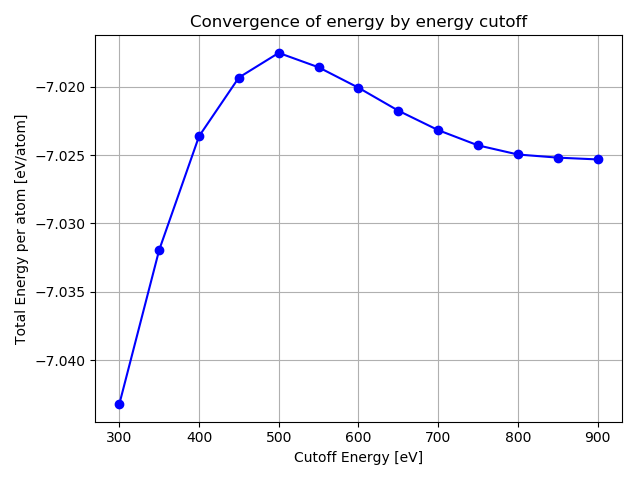
\includegraphics[width = 11cm]{../fig/convergence_energy.png}
      \caption{Plot of energy convergence for Quinizarin, with ENCUT ranging from 300 eV to 900 eV. }
      \label{fig:convergence_energy}
    \end{figure}

    \begin{figure}[H]
      \centering
      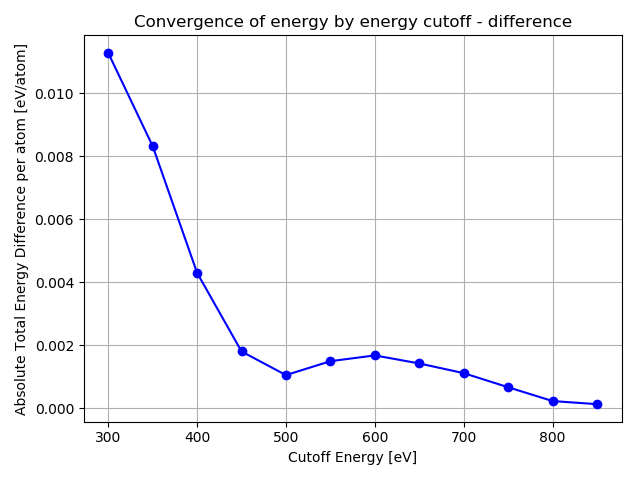
\includegraphics[width = 11cm]{../fig/convergence_energy_difference.png}
      \caption{Plot of the difference in energy convergence for Quinizarin, given by ENCUT. }
      \label{fig:convergence_energy_difference}
    \end{figure}

    \vspace{1cm}

  \subsection{Convergence of k-points}

    For the convergence of k-points the span of values were used as described in Section \ref{sec:Convergence}. Figure~(\ref{fig:convergence_kpoints}) shows how the total energy changes as k-density increases. Like with energy, the difference has also been plotted, and this is shown in Figure~(\ref{fig:convergence_kpoints_difference}).

    \begin{figure}[H]
        \centering
        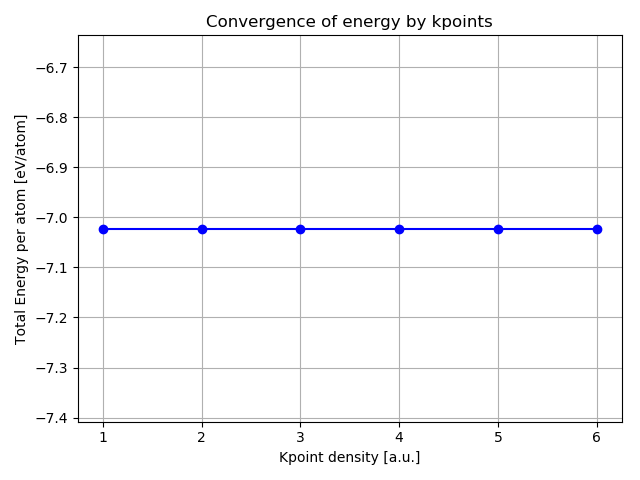
\includegraphics[width = 11cm]{../fig/convergence_kpoints.png}
        \caption{Plot of energy convergence for Quinizarin, with k-point density ranging from 1 to 6. }
        \label{fig:convergence_kpoints}
    \end{figure}

    \begin{figure}[H]
        \centering
        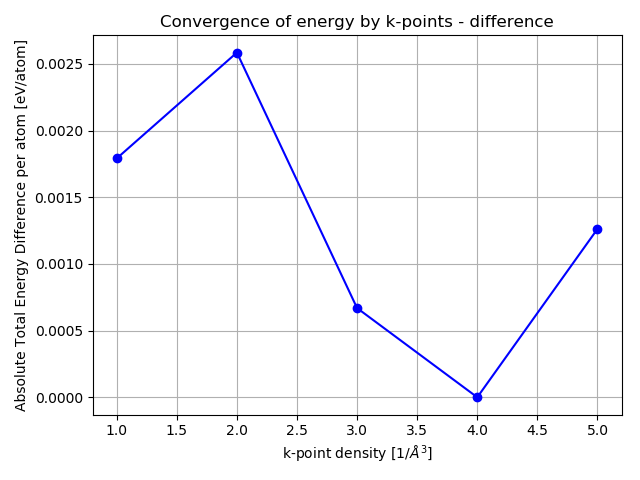
\includegraphics[width = 11cm]{../fig/convergence_kpoints_difference.png}
        \caption{Plot of the difference in energy convergence for Quinizarin, given by k-point density. }
        \label{fig:convergence_kpoints_difference}
    \end{figure}

    \vspace{1cm}

  \subsection{Quinizarin}

    \subsubsection{Relaxing the structure}

      The initial static calculation of Quinizarin gave a CONTCAR as shown in Figure~(\ref{fig:basic_staticbefore_CONTCAR}). \\

      After relaxing the structure and performing a new static calculation, CONTCAR looked as shown in Figure~(\ref{fig:basic_staticafter_CONTCAR}). We do not show CONTCAR from the actual ionic relaxation as it is identical to the post-relaxation static calculation. \\

      Table~(\ref{tab:neighborquinizarin}) shows how the distance between Hydrogen and Oxygen changes from before and after relax. \\

      \begin{figure}[H]
        \centering
        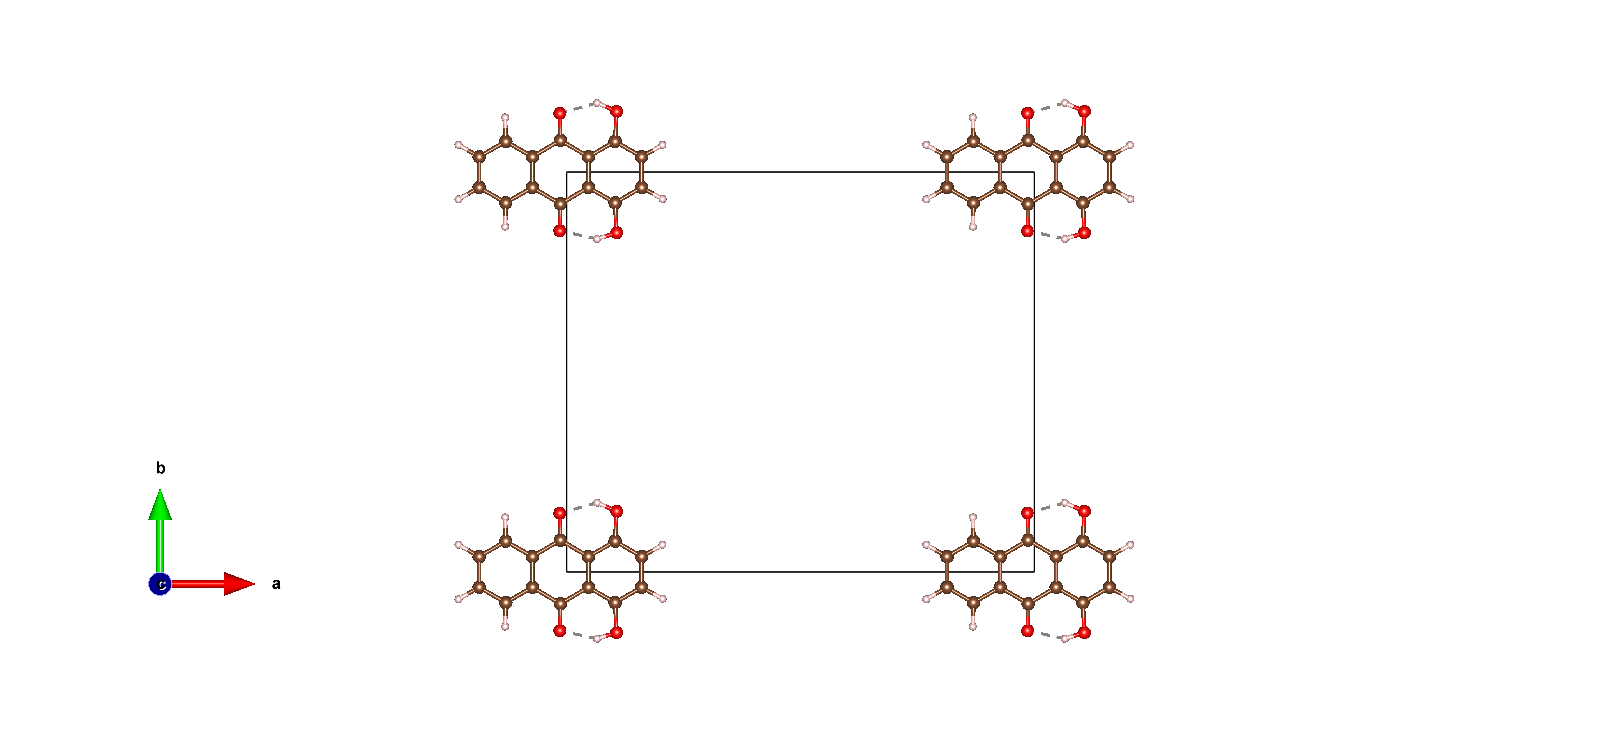
\includegraphics[width = \textwidth]{../fig/basic_staticbefore_CONTCAR.png}
        \caption{Structure of Quinizarin for static VASP calculation. }
        \label{fig:basic_staticbefore_CONTCAR}
      \end{figure}

      \begin{figure}[H]
        \centering
        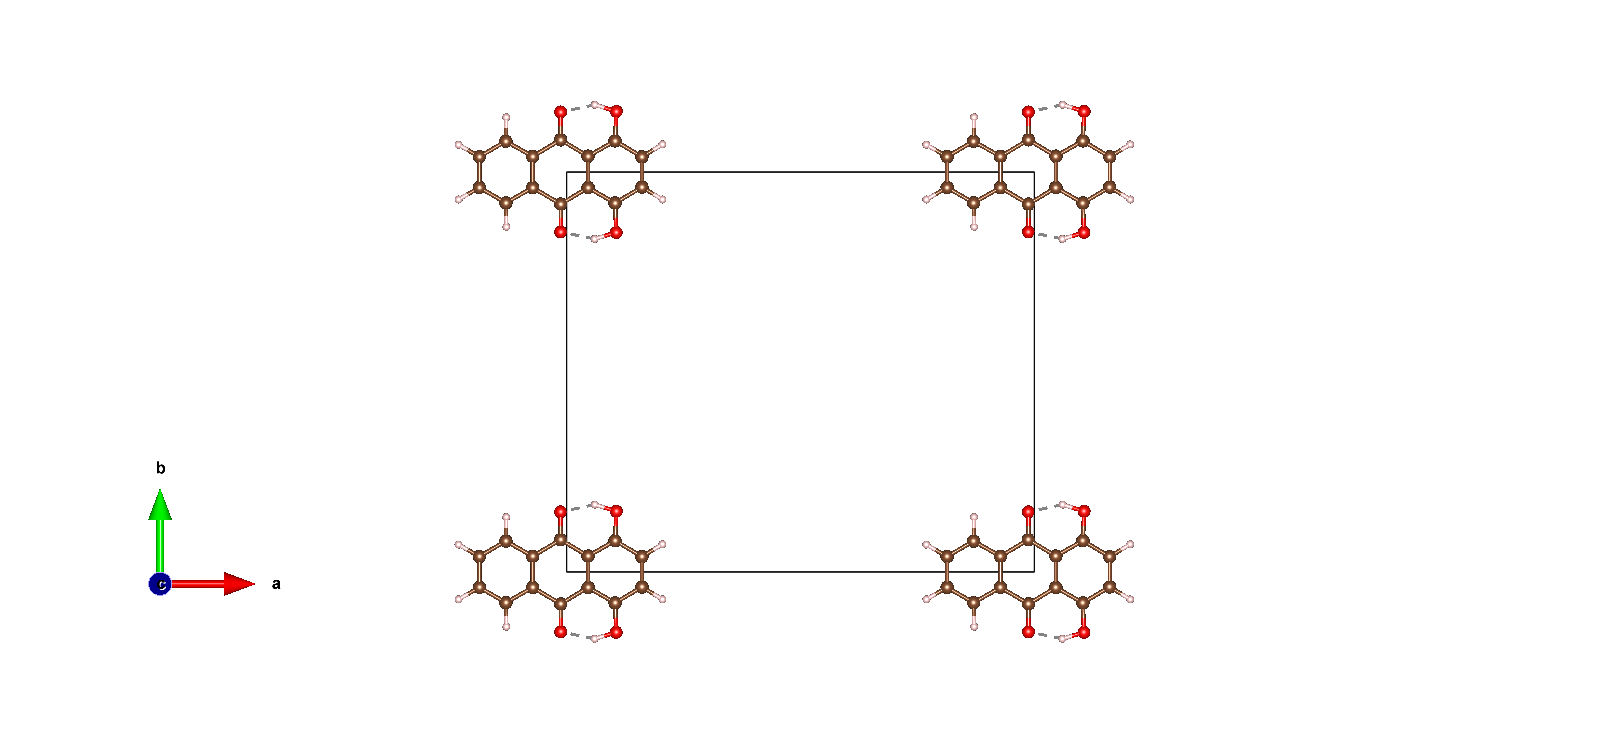
\includegraphics[width = \textwidth]{../fig/basic_staticafter_CONTCAR.png}
        \caption{Structure of Quinizarin for static VASP calculation after relaxed calculation. }
        \label{fig:basic_staticafter_CONTCAR}
      \end{figure}

      \begin{table}[H]
        \centering
        \caption{Hydrogen-Oxygen distances. 2x-bonded Oxygen is the central Oxygen atom, which is has a double bond to carbon. 1x-bonded Oxygen is part of the alcohol-group. The values marked with * were not located in OUTCAR, and so were fetched from VESTA. }
        \label{tab:neighborquinizarin}
        \begin{tabular}{|c|c|c|}
            \hline
            Calculation & Distance to 2x-bonded Oxygen [Å] & Distance to 1x-bonded Oxygen [Å] \\
            \hline \hline
            Before relax lower Hydrogen & $1.73$* & $0.93$ \\
            Before relax upper Hydrogen & $1.76$* & $0.97$ \\
            After relax lower Hydrogen & $1.57$* & $1.03$ \\
            After relax upper Hydrogen & $1.59$* & $1.02$ \\
            \hline
        \end{tabular} \\
        \hspace{0pt}\\
      \end{table}

      \vspace{1cm}

    \subsubsection{Total and relative energies}

      As can be seen in Table~(\ref{tab:TOTENquinizarin}), there was a difference in total energies. This turned out to be -0.015 eV in relative energy difference. The data is taken from static calculations of Quinizarin, before and after a relax VASP calculation. \\

      \begin{table}[H]
        \centering
        \caption{Total energy per atom for Quinizarin with static calculations. }
        \label{tab:TOTENquinizarin}
        \begin{tabular}{|c|c|}
            \hline
            Calculation & Total energy per atom [eV/atom]  \\
            \hline \hline
            Before relax & $-7.019$ \\
            After relax & $-7.034$ \\
            \hline
        \end{tabular} \\
        \hspace{0pt}\\
    \end{table}

      \vspace{1cm}

    \subsubsection{Total and local density of states}

      In Figure~(\ref{fig:basic_TDOS_2}) we can see the total density of states of the Quinizarin molecule. Figure~(\ref{fig:basic_LDOS25_2}) shows the local density of states for the Hydrogen atom in the lower alcohol group, whereas Figure~(\ref{fig:basic_LDOS26_2}) shows the local density of states for the Hydrogen atom in the upper alcohol group. It is important to note that these figures are zoomed in around the Fermi-level.
      To see the full pictures, see Figure~(\ref{fig:basic_TDOS_1}), Figure~(\ref{fig:basic_LDOS25_1}) and Figure~(\ref{fig:basic_LDOS26_1}) in \nameref{sec:Appendix}. \\

      \begin{figure}[H]
        \centering
        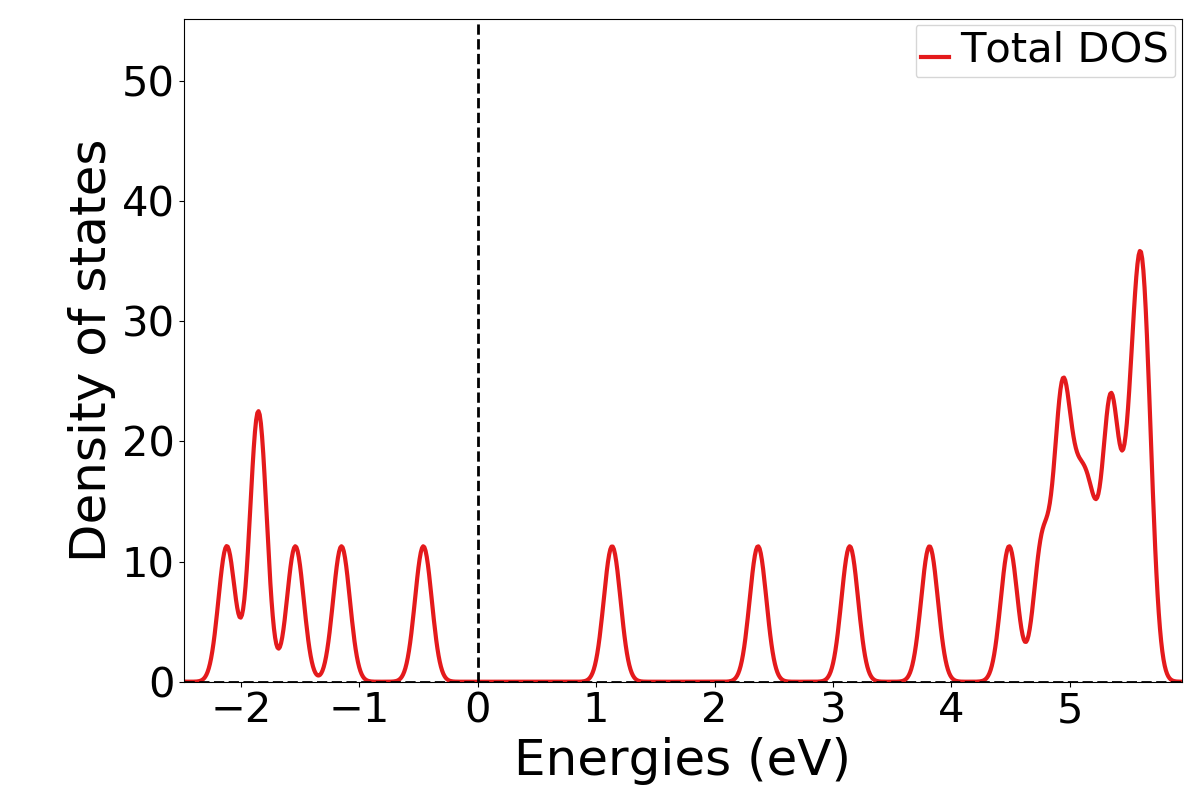
\includegraphics[width = 11cm]{../fig/basic_TDOS_2.png}
        \caption{Plot of total DOS for Quinizarin, zoomed in for energies around the fermi level (set to 0 eV). }
        \label{fig:basic_TDOS_2}
      \end{figure}

      \begin{figure}[H]
        \centering
        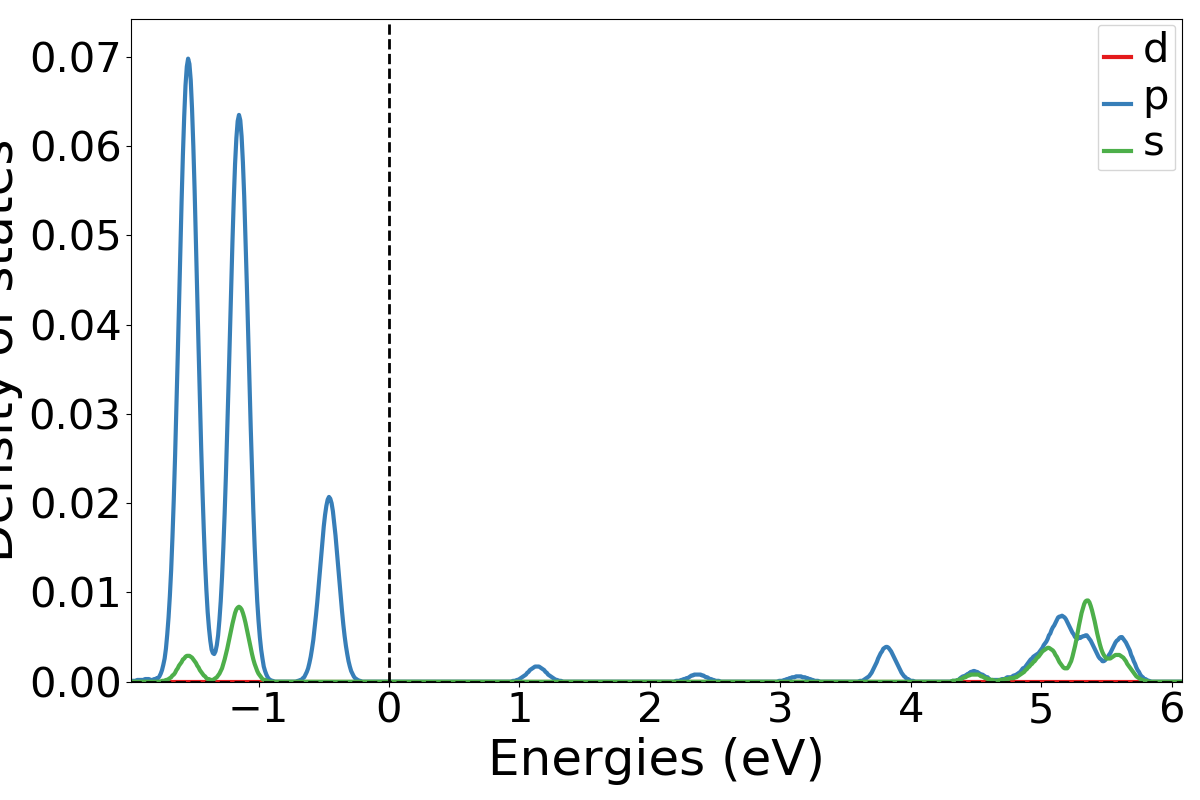
\includegraphics[width = 11cm]{../fig/basic_LDOS25_2.png}
        \caption{Plot of local DOS for atom number 25(H in alcohol-group) for Quinizarin, zoomed in for energies around the fermi level (set to 0 eV). }
        \label{fig:basic_LDOS25_2}
      \end{figure}

      \begin{figure}[H]
        \centering
        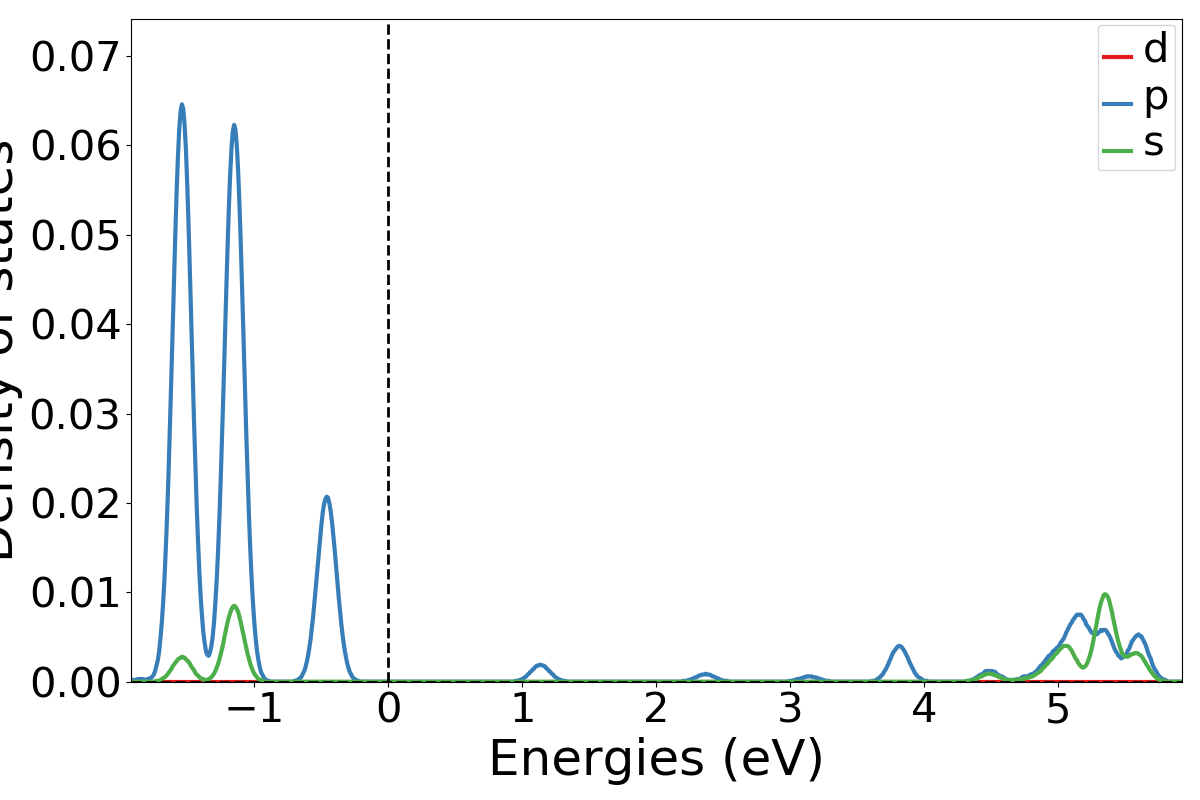
\includegraphics[width = 11cm]{../fig/basic_LDOS26_2.png}
        \caption{Plot of local DOS for atom number 26(H in alcohol-group) for Quinizarin, zoomed in for energies around the fermi level (set to 0 eV). }
        \label{fig:basic_LDOS26_2}
      \end{figure}

      \vspace{1cm}

    \subsubsection{Band gap}

      Table (\ref{tab:bandgapquinizarin}) below shows the band gap, the valance band maximum (VBM), and the conduction band minimum (CBM) for Quinizarin, before and after a relax calculation, using static calculations. \\

      \begin{table}[H]
        \centering
        \caption{Band gap, valance band maximum and conduction band minimum for Quinizarin with static calculations. }
        \label{tab:bandgapquinizarin}
        \begin{tabular}{|c|c|c|c|}
            \hline
            Calculation & Band gap [eV] & VBM [eV] & CBM [eV]  \\
            \hline \hline
            Before relax & $1.773$ & $-5.335$ & $-3.562$ \\
            After relax & $1.594$ & $-5.313$ & $-3.720$ \\
            \hline
        \end{tabular} \\
        \hspace{0pt}\\
      \end{table}

      \vspace{1cm}

    \subsubsection{Charge density}

      The charge density before relaxation is shown in Figure~(\ref{fig:basic_staticbefore_CHGCAR}). The charge density for the static calculation after relaxation can be shown in Figure~(\ref{fig:basic_staticafter_CHGCAR}).
      Figure~(\ref{fig:basic_staticafter_CHGDENSITY}) shows the charge density of a single molecule after having relaxed the structure. \\

      \begin{figure}[H]
        \centering
        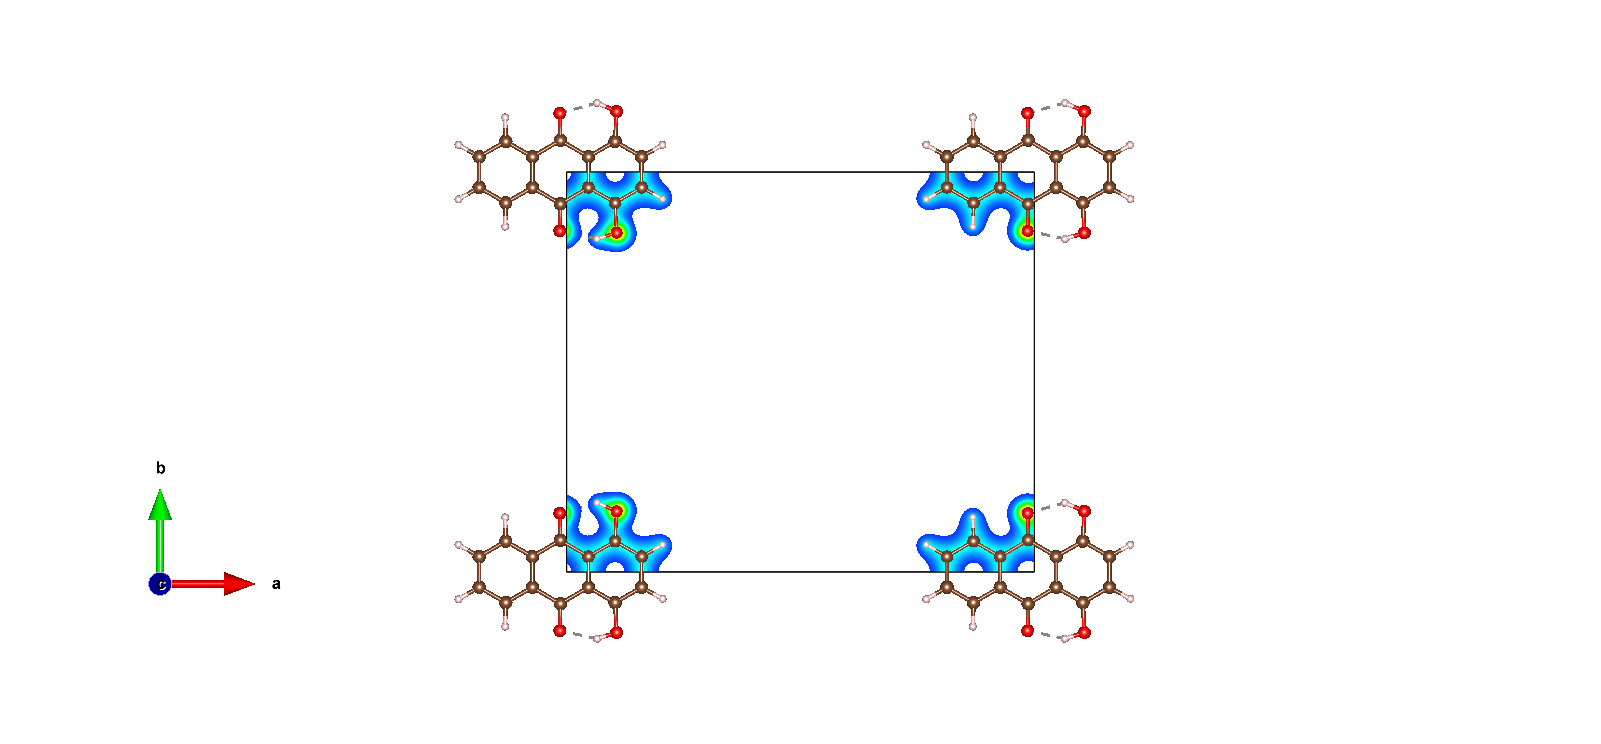
\includegraphics[width = \textwidth]{../fig/basic_staticbefore_CHGCAR.png}
        \caption{Charge density of Quinizarin for static VASP calculation. }
        \label{fig:basic_staticbefore_CHGCAR}
      \end{figure}

      \begin{figure}[H]
        \centering
        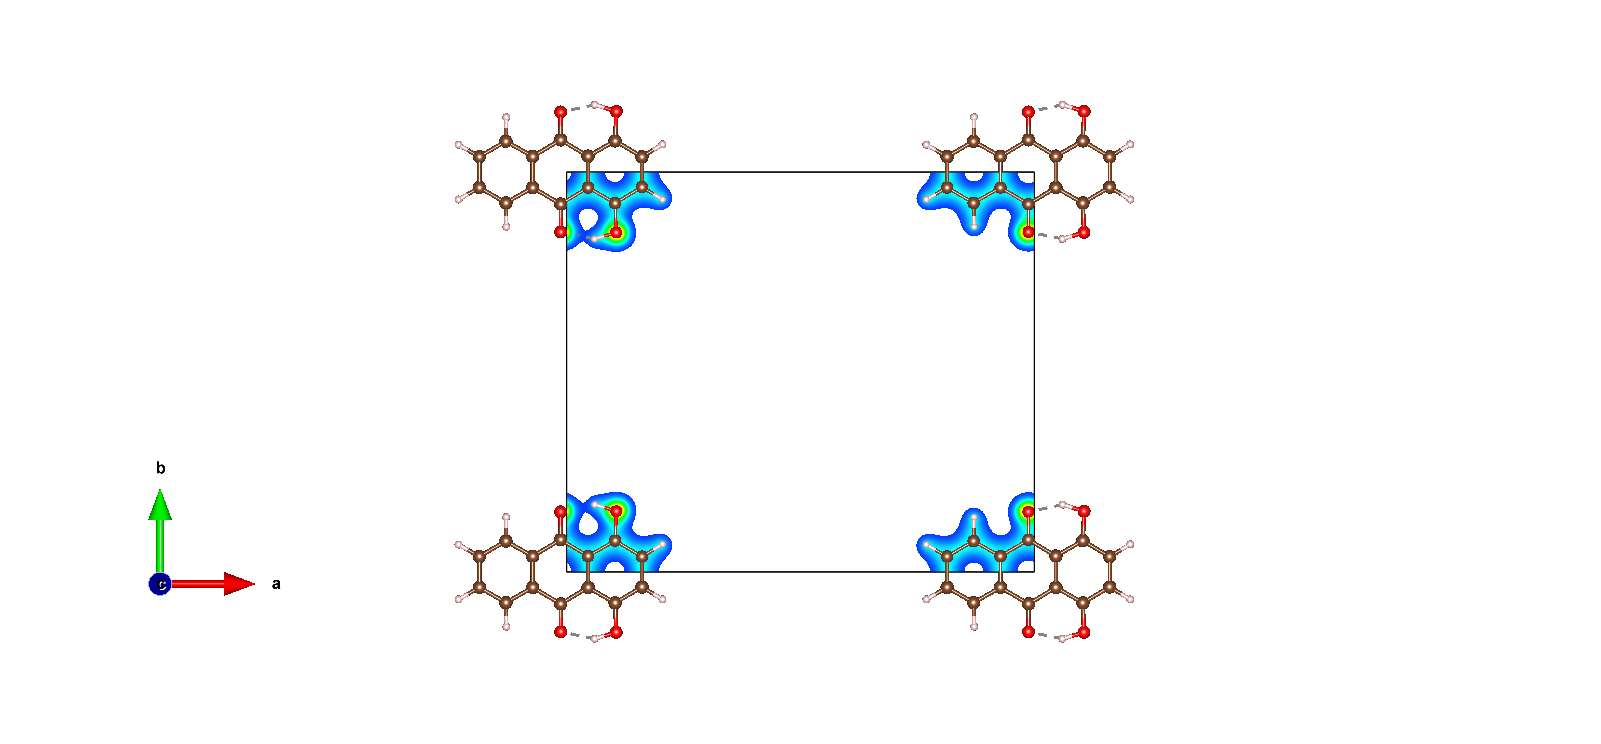
\includegraphics[width = \textwidth]{../fig/basic_staticafter_CHGCAR.png}
        \caption{Charge density of Quinizarin for static VASP calculation after relaxed calculation. }
        \label{fig:basic_staticafter_CHGCAR}
      \end{figure}

      \begin{figure}[H]
        \centering
        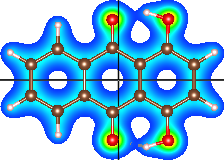
\includegraphics[width = 5cm]{../fig/basic_staticafter_CHGDENSITY.png}
        \caption{Charge density of a single Quinizarin molecule for static VASP calculation after relaxed calculation. }
        \label{fig:basic_staticafter_CHGDENSITY}
      \end{figure}

      \vspace{1cm}

  \subsection{Quinizarin with Yttrium}

    \subsubsection{Relaxing the structure}

      Below we can see the structure of Quinizarin with Yttrium. Figure~(\ref{fig:Y_staticbefore_CONTCAR}) shows it as it is before relaxing the structure, and Figure (\ref{fig:Y_staticafter_CONTCAR}) shows the structure after having been relaxed. \\

      In Table~(\ref{tab:neighborY}) we can see Yttrium's distance to oxygen, both before and after relaxing the structures. \\

      \begin{figure}[H]
        \centering
        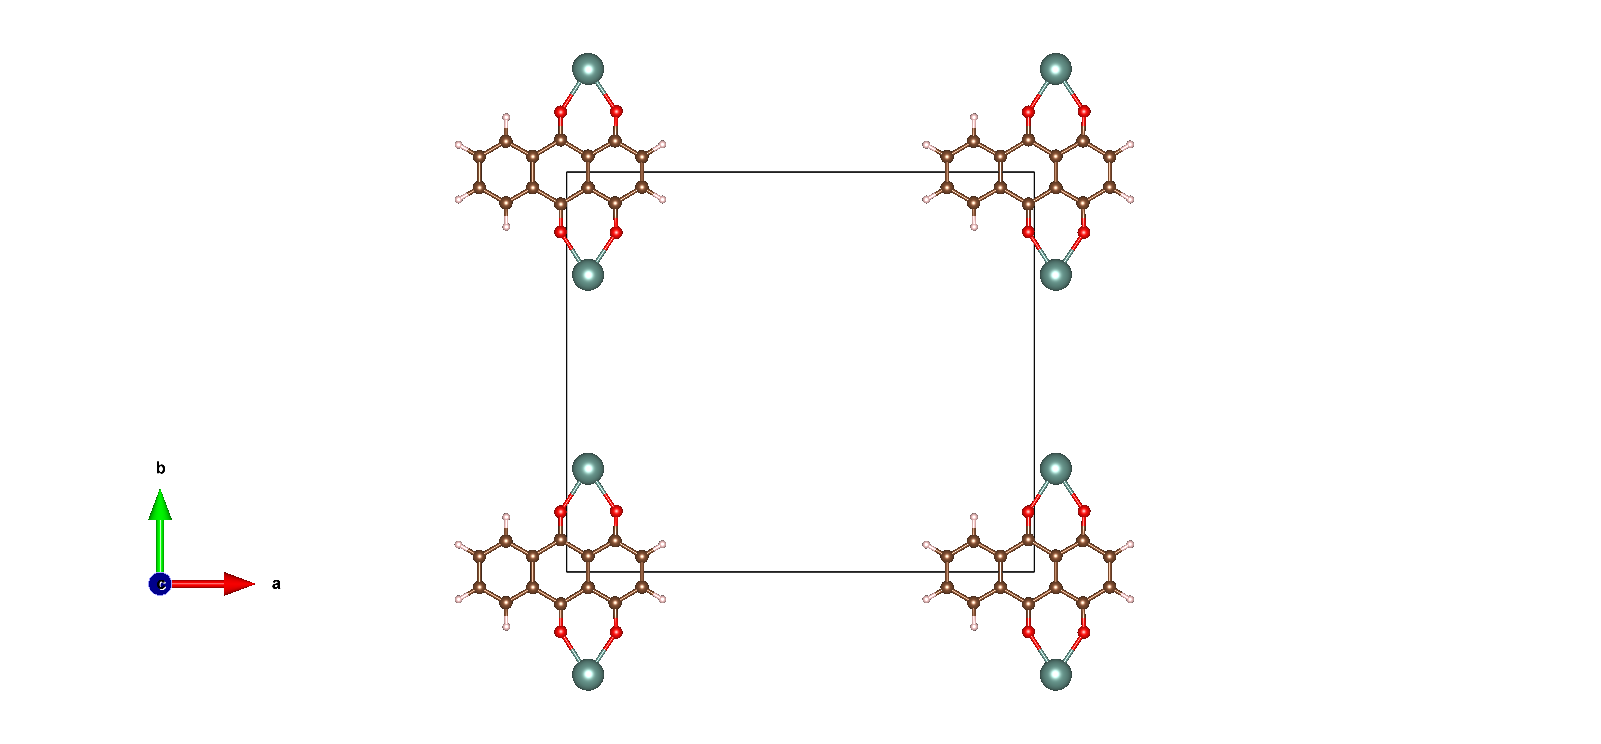
\includegraphics[width = \textwidth]{../fig/Y_staticbefore_CONTCAR.png}
        \caption{Structure of Quinizarin with Yttrium for static VASP calculation. }
        \label{fig:Y_staticbefore_CONTCAR}
      \end{figure}

      \begin{figure}[H]
        \centering
        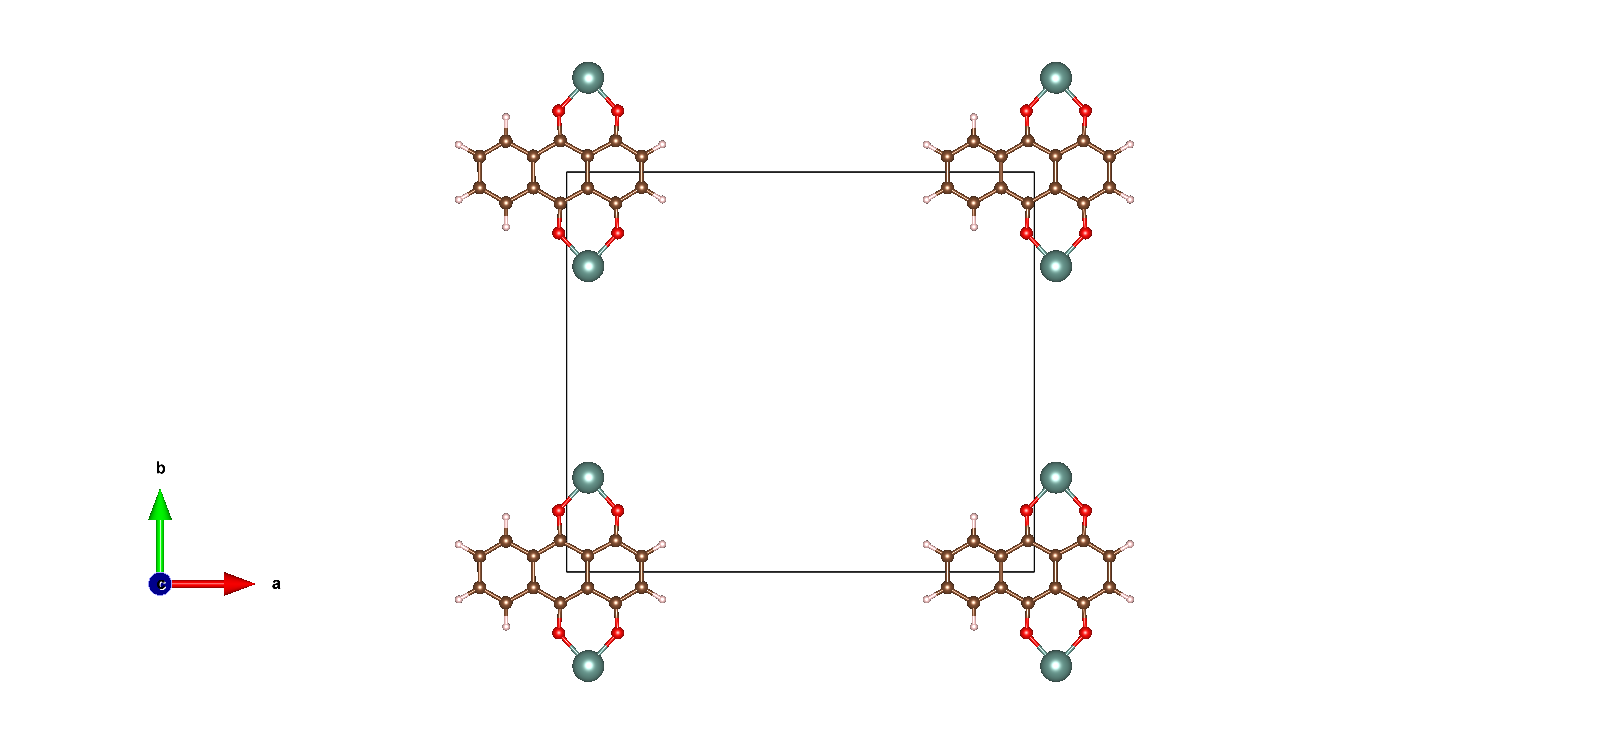
\includegraphics[width = \textwidth]{../fig/Y_staticafter_CONTCAR.png}
        \caption{Structure of Quinizarin with Yttrium for static VASP   calculation after relaxed calculation. }
        \label{fig:Y_staticafter_CONTCAR}
      \end{figure}

      \begin{table}[H]
        \centering
        \caption{Yttrium-Oxygen distances. 2x-bonded Oxygen is the central Oxygen atom, which is has a double bond to carbon. 1x-bonded Oxygen is part of the alcohol-group. }
        \label{tab:neighborY}
        \begin{tabular}{|c|c|c|}
            \hline
            Calculation & Distance to 2x-bonded Oxygen [Å] & Distance to 1x-bonded Oxygen [Å]  \\
            \hline \hline
            Before relax lower Yttrium & $2.32$ & $2.31$ \\
            Before relax upper Yttrium & $2.32$ & $2.32$ \\
            After relax lower Yttrium & $2.02$ & $2.01$ \\
            After relax upper Yttrium & $2.02$ & $2.01$ \\
            \hline
        \end{tabular} \\
        \hspace{0pt}\\
      \end{table}

      \vspace{1cm}

    \subsubsection{Total and relative energies}

      Table~(\ref{tab:TOTENY}) shows the total energy per atom for Quinizarin with Yttrium, with calculations done by static calculations before and after a relax calculation. The relative energy was $-0.109$ eV/atom. \\

      \begin{table}[H]
        \centering
        \caption{Total energy per atom for Quinizarin with Yttrium. }
        \vspace{0mm}
        \label{tab:TOTENY}
        \begin{tabular}{|c|c|}
            \hline
            Calculation & Total energy per atom [eV/atom]  \\
            \hline \hline
            Before relax & $-7.167$ \\
            After relax & $-7.276$ \\
            \hline
        \end{tabular} \\
        \hspace{0pt}\\
      \end{table}

      \vspace{1cm}

    \subsubsection{Total and local density of states}

      TDOS and LDOS graphs are shown below. Figure~(\ref{fig:Y_TDOS_2}) shows the total DOS for Quinizarin with Yttrium, whilst Figure~(\ref{fig:Y_LDOS25_2}) shows the local DOS for the lower Yttrium atom and Figure~(\ref{fig:Y_LDOS25_2}) shows the local DOS for the upper Yttrium atom.
      The full pictures of these plots, see Figure (\ref{fig:Y_TDOS_1}), Figure (\ref{fig:Y_LDOS25_1}) and Figure (\ref{fig:Y_LDOS26_1}) in \nameref{sec:Appendix}. \\

      \begin{figure}[H]
        \centering
        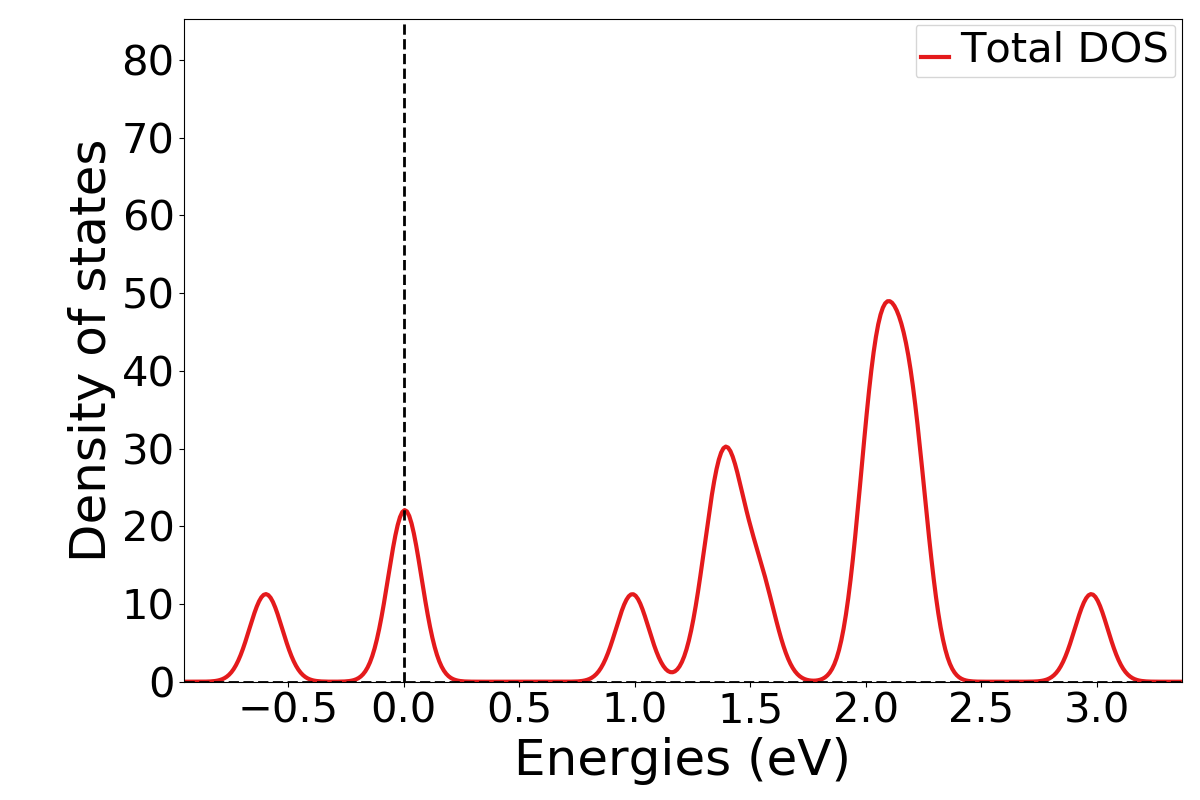
\includegraphics[width = 11cm]{../fig/Y_TDOS_2.png}
        \caption{Plot of total DOS for Yttrium, zoomed in for energies around the fermi level (set to 0 eV). }
        \label{fig:Y_TDOS_2}
      \end{figure}

      \begin{figure}[H]
        \centering
        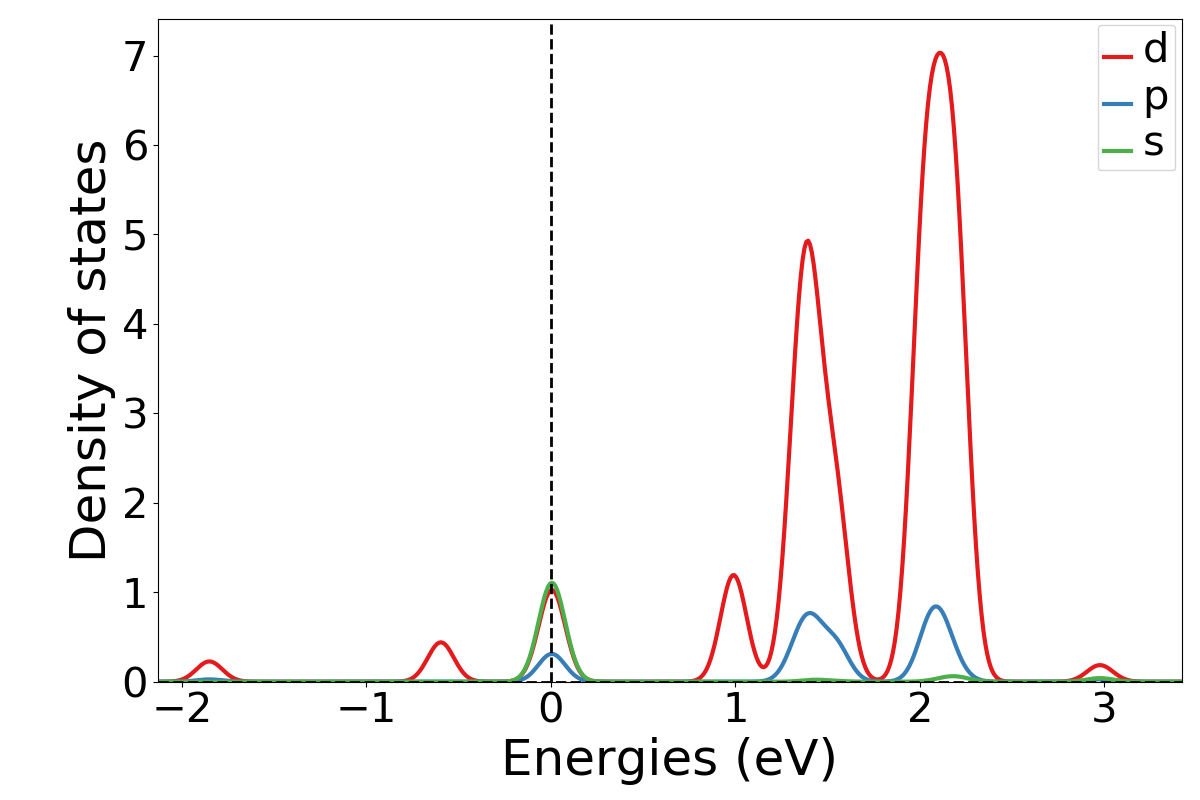
\includegraphics[width = 11cm]{../fig/Y_LDOS25_2.png}
        \caption{Plot of local DOS of atom number 25(Y in lower alcohol-group) for Quinizarin with Yttrium, zoomed in for energies around the fermi level (set to 0 eV). }
        \label{fig:Y_LDOS25_2}
      \end{figure}

      \begin{figure}[H]
          \centering
          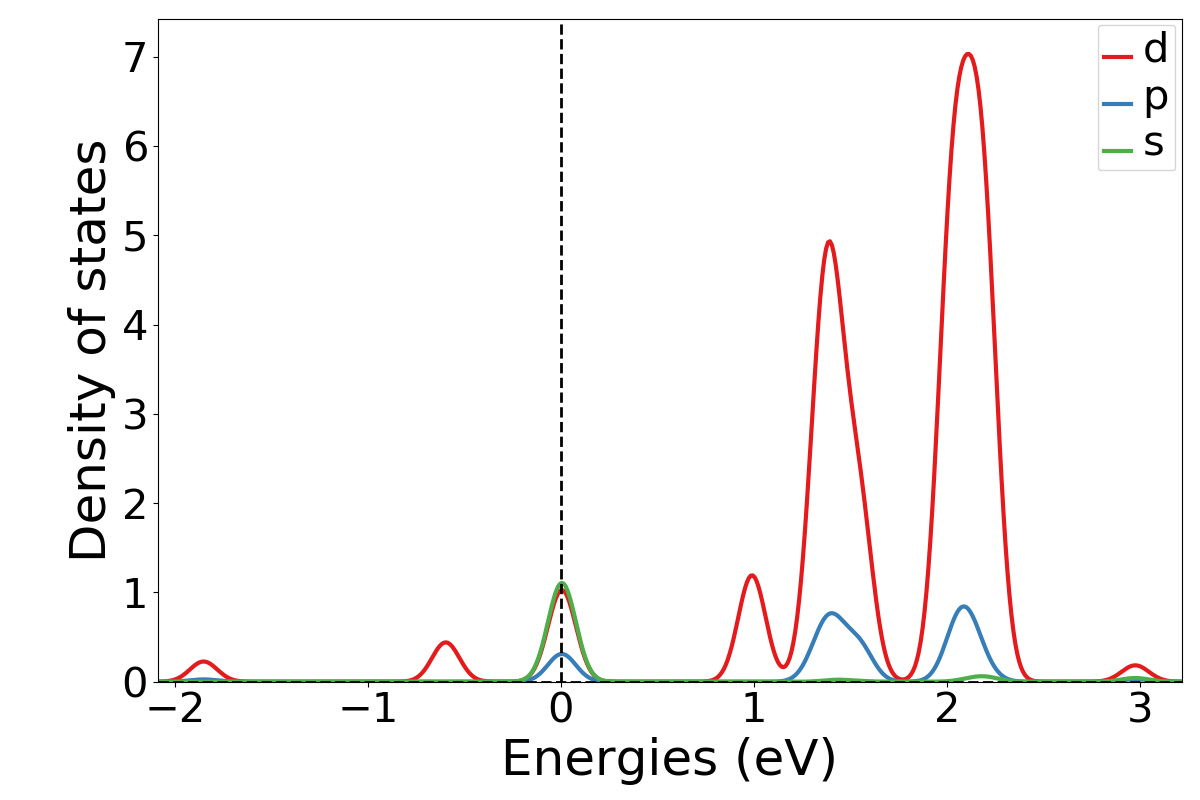
\includegraphics[width = 11cm]{../fig/Y_LDOS26_2.png}
          \caption{Plot of local DOS of atom number 26(Y in upper alcohol-group) for Quinizarin with Yttrium, zoomed in for energies around the fermi level (set to 0 eV). }
          \label{fig:Y_LDOS26_2}
      \end{figure}

      \vspace{1cm}

    \subsubsection{Band gap}

      The table below, Table~(\ref{tab:bandgapY}), shows the values of the band gap of Quinizarin with Yttrium. It also shows how the values between before and after relaxing the structure. \\

      \begin{table}[H]
        \centering
        \caption{Band gap, valance band maximum and conduction band minimum for Quinizarin with Yttrium with static calculations. }
        \vspace{0mm}
        \label{tab:bandgapY}
        \begin{tabular}{|c|c|c|c|}
            \hline
            Calculation & Band gap [eV] & VBM [eV] & CBM [eV]  \\
            \hline \hline
            Before relax & $0.042$ & $-3.323$ & $-3.281$ \\
            After relax & $0.029$ & $-2.979$ & $-2.950$ \\
            \hline
        \end{tabular} \\
        \hspace{0pt}\\
      \end{table}

      \vspace{1cm}

    \subsubsection{Charge density}

      Figure~(\ref{fig:Y_staticbefore_CHGCAR}) and Figure~(\ref{fig:Y_staticafter_CHGCAR}) show the charge density of Quinizarin with Yttrium, respectively before and after relaxation. Figure~(\ref{fig:basic_staticafter_CHGDENSITY}) shows the charge density of a single molecule of Quinizarin with Yttrium after relaxation. \\

      \begin{figure}[H]
        \centering
        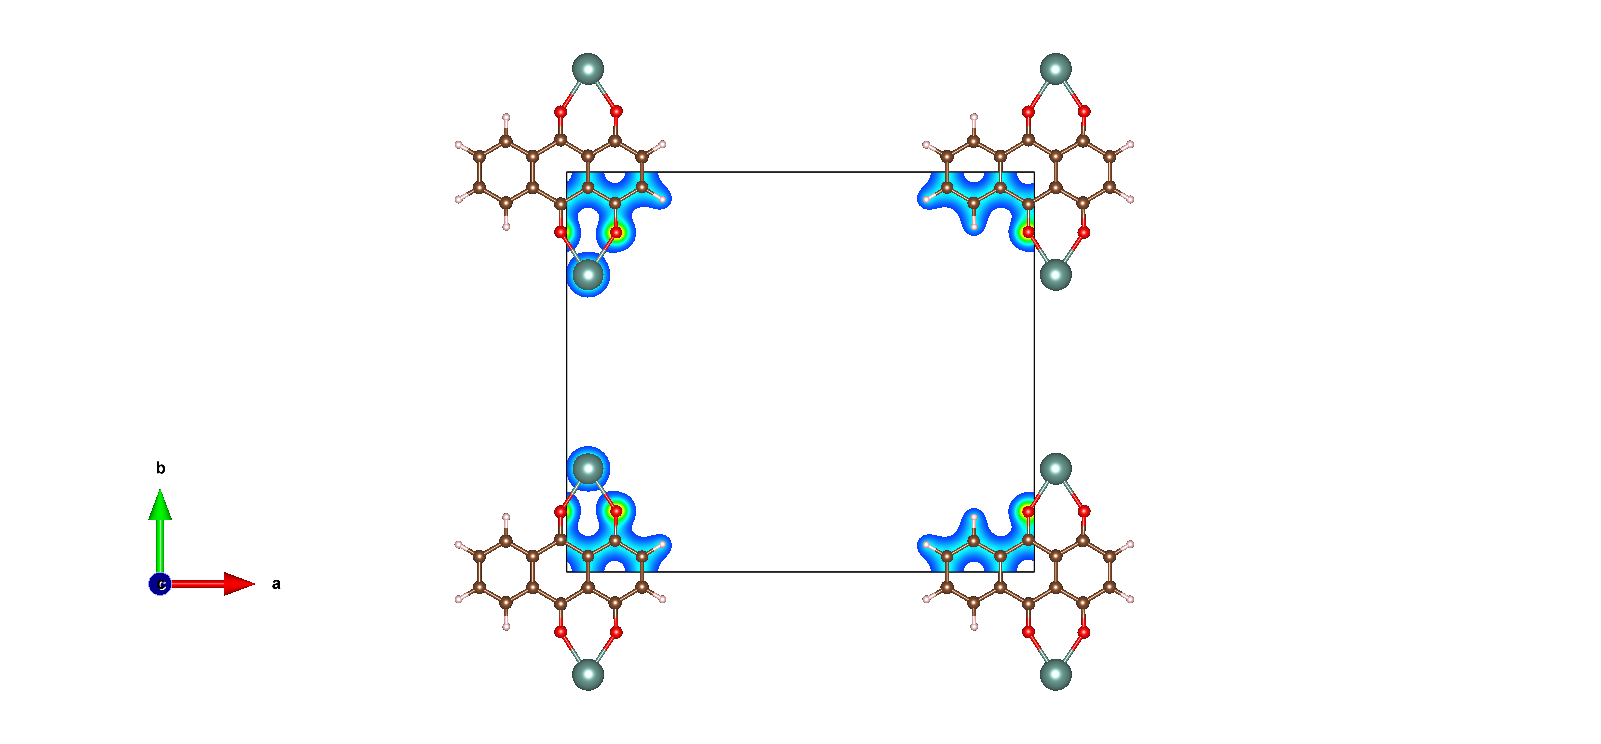
\includegraphics[width = \textwidth]{../fig/Y_staticbefore_CHGCAR.png}
        \caption{Charge density of Quinizarin with Yttrium for static VASP calculation. }
        \label{fig:Y_staticbefore_CHGCAR}
      \end{figure}

      \begin{figure}[H]
        \centering
        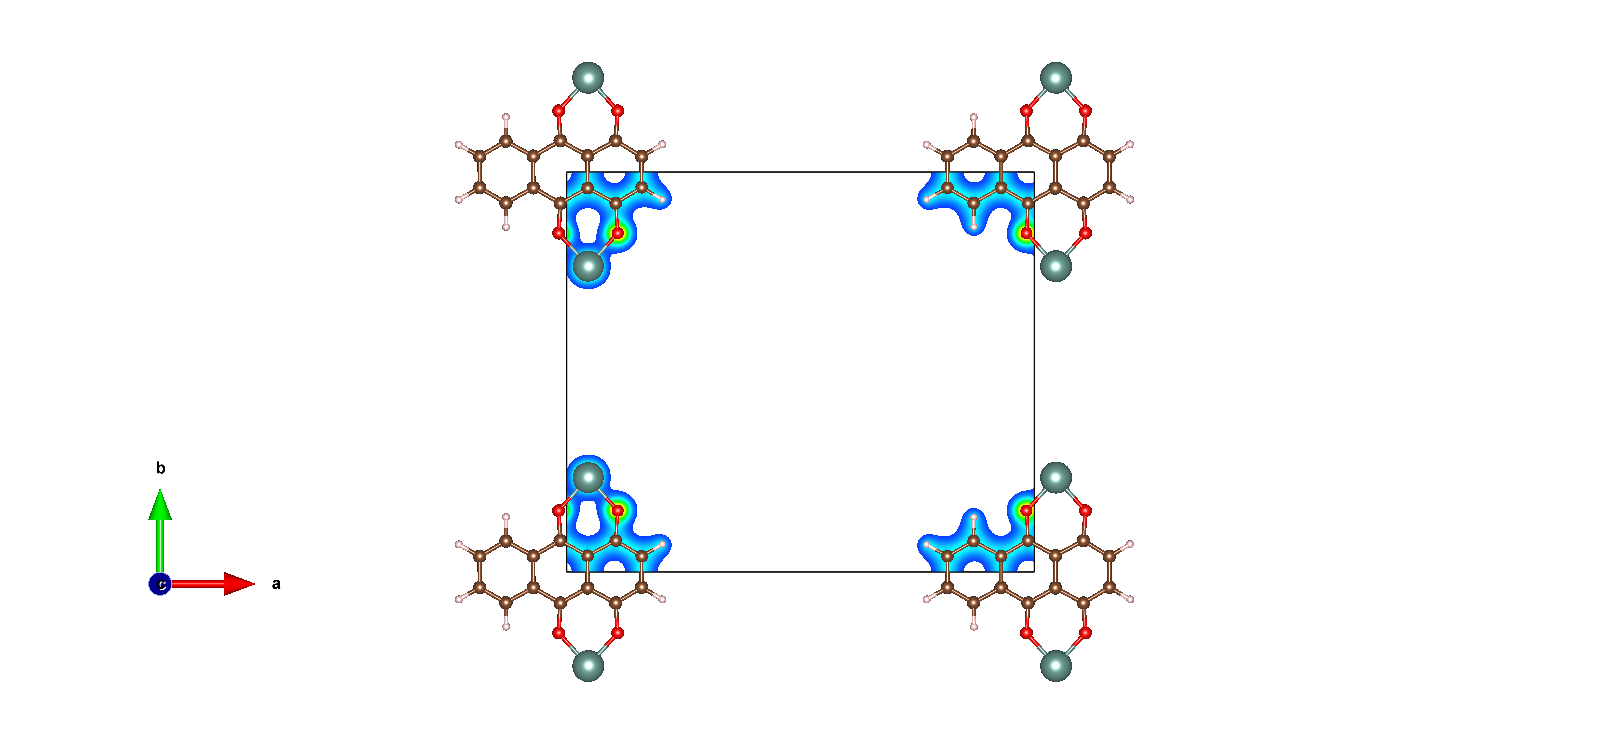
\includegraphics[width = \textwidth]{../fig/Y_staticafter_CHGCAR.png}
        \caption{Charge density of Quinizarin with Yttrium for static VASP calculation after relaxed calculation. }
        \label{fig:Y_staticafter_CHGCAR}
      \end{figure}

      \begin{figure}[H]
        \centering
        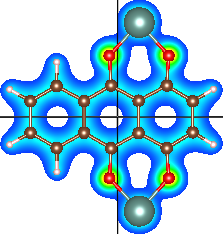
\includegraphics[width = 5cm]{../fig/Y_staticafter_CHGDENSITY.png}
        \caption{Charge density of a single Quinizarin molecule with Yttrium for static VASP calculation after relaxed calculation. }
        \label{fig:Y_staticafter_CHGDENSITY}
      \end{figure}

      \vspace{1cm}

  \subsection{Quinizarin with Ytterbium}

    \subsubsection{Relaxing the structure}

      Quinizarin with Ytterbium before relaxation is shown in Figure~(\ref{fig:Yb_staticbefore_CONTCAR}). After relaxation the structure looked as in Figure~(\ref{fig:Yb_staticafter_CONTCAR}). \\

      OUTCAR can display the nearest neighbors, which is the atomic distance between the atoms in the structure. In Table~(\ref{tab:neighborYb}) below, the Ytterbium and Oxygen distances is shown. \\

      \begin{figure}[H]
        \centering
        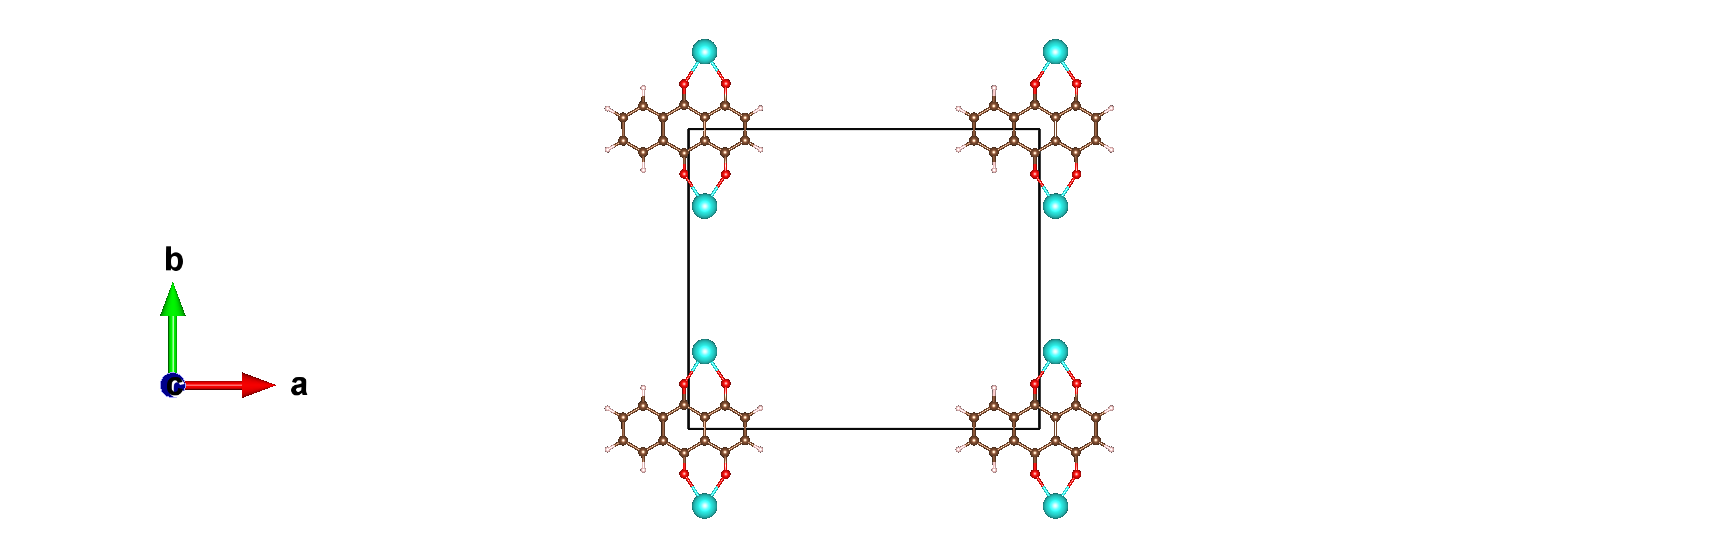
\includegraphics[width = \textwidth]{../fig/Yb_staticbefore_CONTCAR.png}
        \caption{Structure of Quinizarin with Ytterbium for static VASP calculation. }
        \label{fig:Yb_staticbefore_CONTCAR}
      \end{figure}

      \begin{figure}[H]
        \centering
        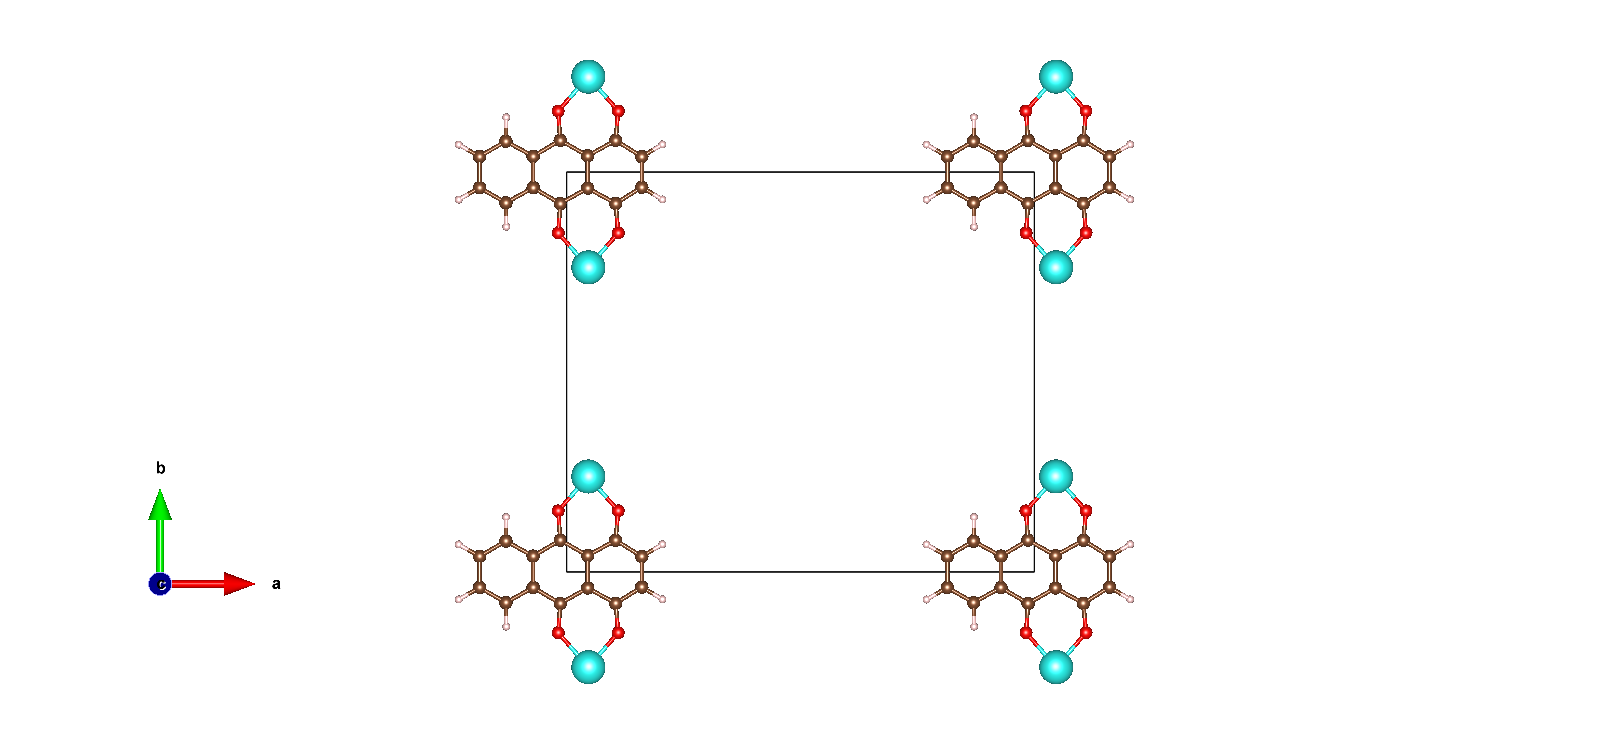
\includegraphics[width = \textwidth]{../fig/Yb_staticafter_CONTCAR.png}
        \caption{Structure of Quinizarin with Ytterbium for static VASP calculation after relaxed calculation. }
        \label{fig:Yb_staticafter_CONTCAR}
      \end{figure}

      \begin{table}[H]
        \centering
        \caption{Ytterbium-Oxygen distances. 2x-bonded Oxygen is the central Oxygen atom, which is has a double bond to carbon. 1x-bonded Oxygen is part of the alcohol-group. }
        \label{tab:neighborYb}
        \begin{tabular}{|c|c|c|}
            \hline
            Calculation & Distance to 2x-bonded Oxygen [Å] & Distance to 1x-bonded Oxygen [Å]  \\
            \hline \hline
            Before relax lower Ytterbium & $2.32$ & $2.31$ \\
            Before relax upper Ytterbium & $2.32$ & $2.32$ \\
            After relax lower Ytterbium & $2.08$ & $2.07$ \\
            After relax upper Ytterbium & $2.08$ & $2.07$ \\
            \hline
        \end{tabular} \\
        \hspace{0pt}\\
      \end{table}


      \vspace{1cm}

    \subsubsection{Total and relative energies}

      See Table~(\ref{tab:TOTENYb}) for a table comparing the total energies of the static VASP calculations of Quinizarin with Ytterbium. The relative energy was $-0.013$ eV difference. \\

      \begin{table}[H]
        \centering
        \caption{Total energy per atom for Quinizarin with Ytterbium before and after relaxation. }
        \label{tab:TOTENYb}
        \begin{tabular}{|c|c|}
            \hline
            Calculation & Total energy per atom [eV/atom]  \\
            \hline \hline
            Before relax & $-6.869$ \\
            After relax & $-6.882$ \\
            \hline
        \end{tabular} \\
        \hspace{0pt}\\
      \end{table}

      \vspace{1cm}

    \subsubsection{Total and local density of states}

      Figure~(\ref{fig:Yb_TDOS_2}) shows the total DOS of Quinizarin with Ytterbium. Figure~(\ref{fig:Yb_LDOS25_3}) and Figure~(\ref{fig:Yb_LDOS26_3}) respectively show the local DOS of the lower and upper Ytterbium atoms. The f-orbital is cut of due to being so high (around 50).
      In addition, to see the uncropped figures, see Figure~(\ref{fig:Yb_TDOS_1}), Figure~(\ref{fig:Yb_LDOS25_1}) and Figure~(\ref{fig:Yb_LDOS26_1}) in \nameref{sec:Appendix}.\\

      \begin{figure}[H]
        \centering
        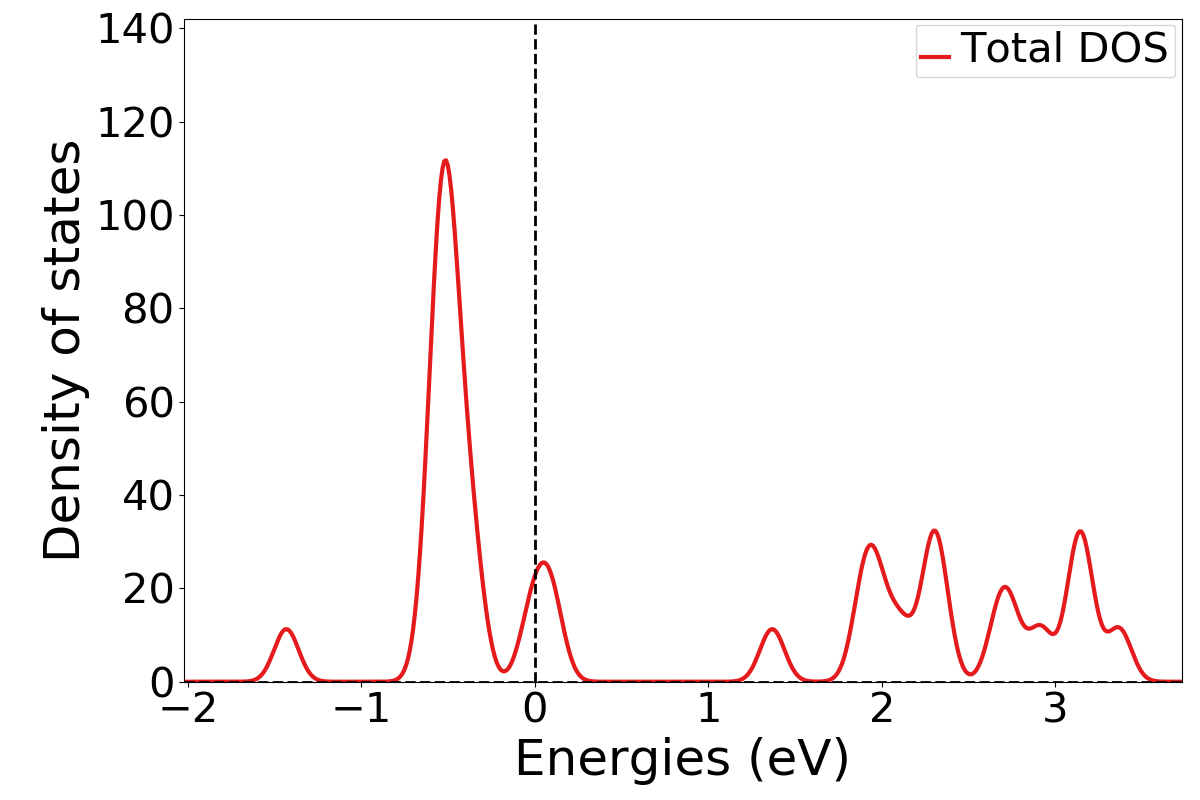
\includegraphics[width = 11cm]{../fig/Yb_TDOS_2.png}
        \caption{Plot of total DOS for Ytterbium, zoomed in for energies around the fermi level (set to 0 eV). }
        \label{fig:Yb_TDOS_2}
      \end{figure}

      \begin{figure}[H]
          \centering
          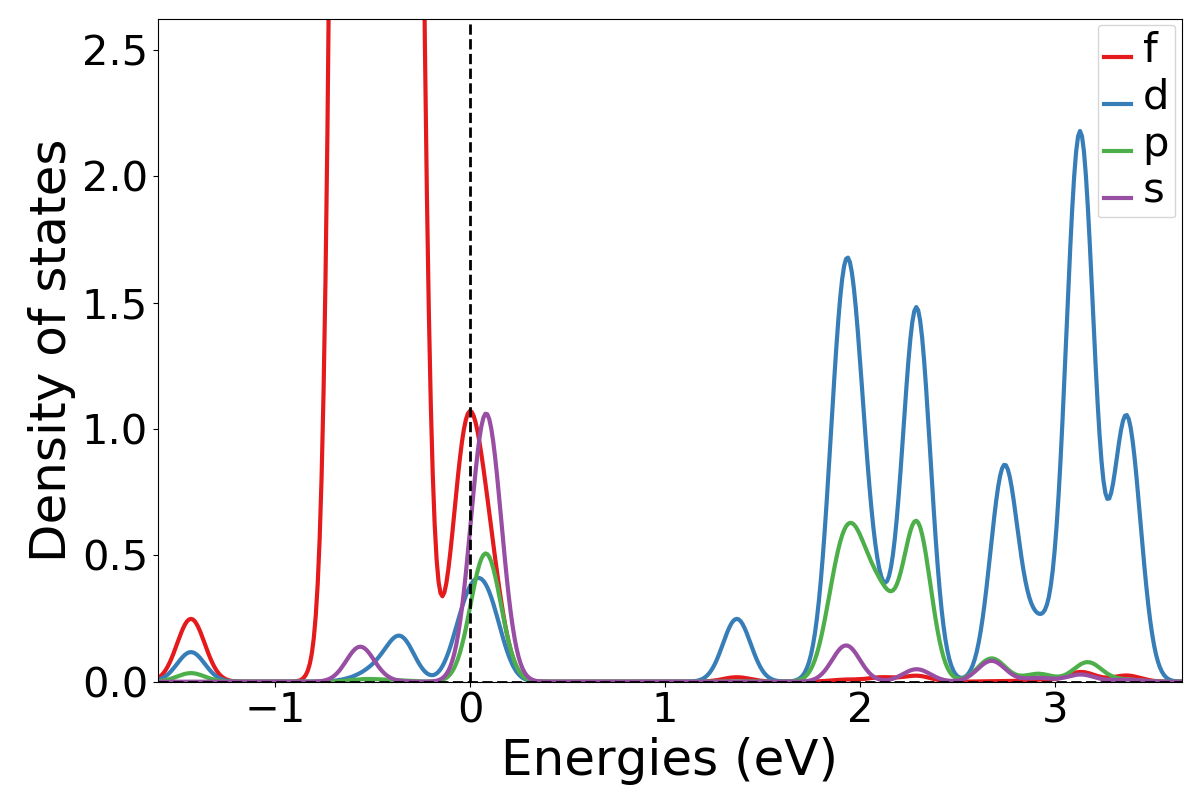
\includegraphics[width = 11cm]{../fig/Yb_LDOS25_3.png}
          \caption{Plot of local DOS of atom number 25(Yb in lower alcohol-group) for Quinizarin with Ytterbium, zoomed in for energies around the fermi level (set to 0 eV). }
          \label{fig:Yb_LDOS25_3}
      \end{figure}

      \begin{figure}[H]
          \centering
          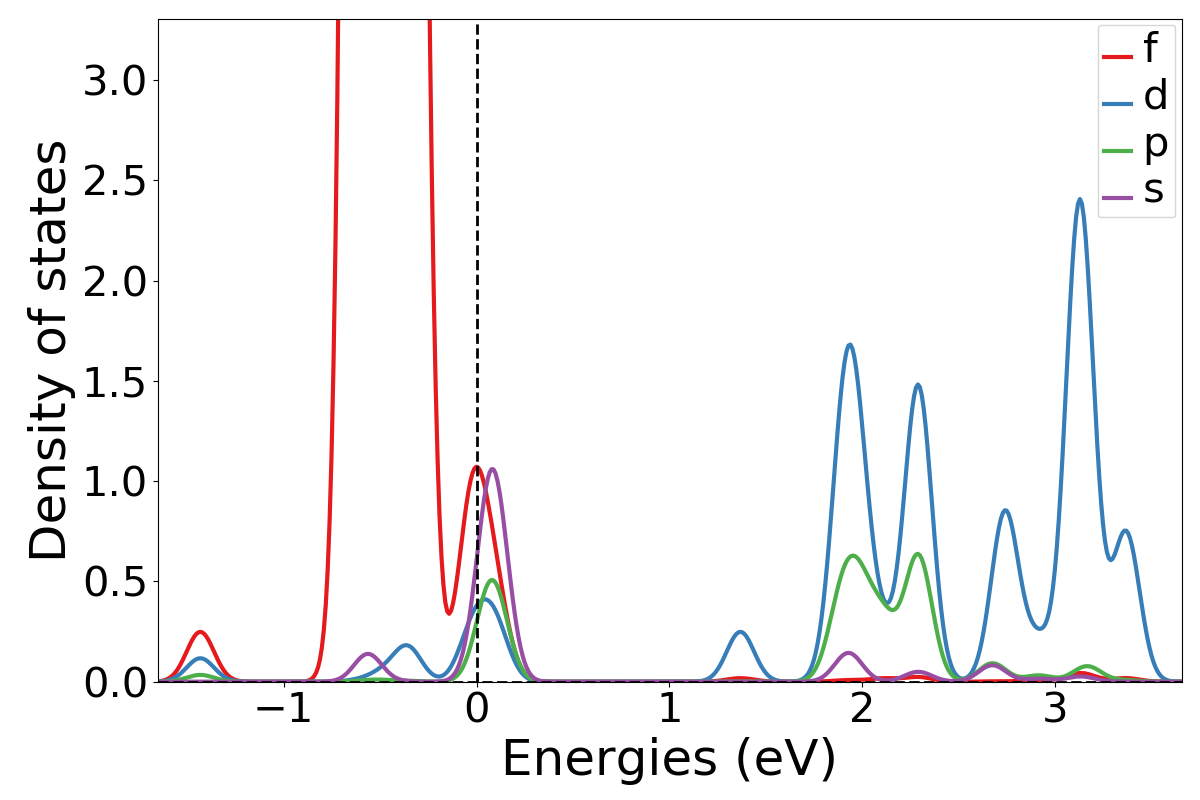
\includegraphics[width = 11cm]{../fig/Yb_LDOS26_3.png}
          \caption{Plot of local DOS of atom number 26(Yb in upper alcohol-group) for Quinizarin with Ytterbium, zoomed in for energies around the fermi level (set to 0 eV). }
          \label{fig:Yb_LDOS26_3}
      \end{figure}

      \vspace{1cm}

    \subsubsection{Band gap}

      Table~(\ref{tab:bandgapYb}) shows the band gap of Quinizarin with Ytterbium using static VASP calculations, both before and after relaxing the structure. \\

      \begin{table}[H]
        \centering
        \caption{Band gap, valance band maximum and conduction band minimum for Quinizarin with Ytterbium with static calculations. }
        \vspace{0mm}
        \label{tab:bandgapYb}
        \begin{tabular}{|c|c|c|c|}
            \hline
            Calculation & Band gap [eV] & VBM [eV] & CBM [eV]  \\
            \hline \hline
            Before relax & $0.0552$ & $-2.9157$ & $-2.6422$ \\
            After relax & $0.0771$ & $-2.7193$ & $-3.720$ \\
            \hline
        \end{tabular} \\
        \hspace{0pt}\\
      \end{table}

      \vspace{1cm}

    \subsubsection{Charge density}

      Figure~(\ref{fig:Yb_staticbefore_CHGCAR}) and Figure~(\ref{fig:Yb_staticafter_CHGCAR}) show the charge density of Quinizarin with Ytterbium respectively before and after relaxation. Figure~(\ref{fig:Yb_staticafter_CHGDENSITY}) show the charge density of a single molecule, also after relaxation. \\

      \begin{figure}[H]
          \centering
          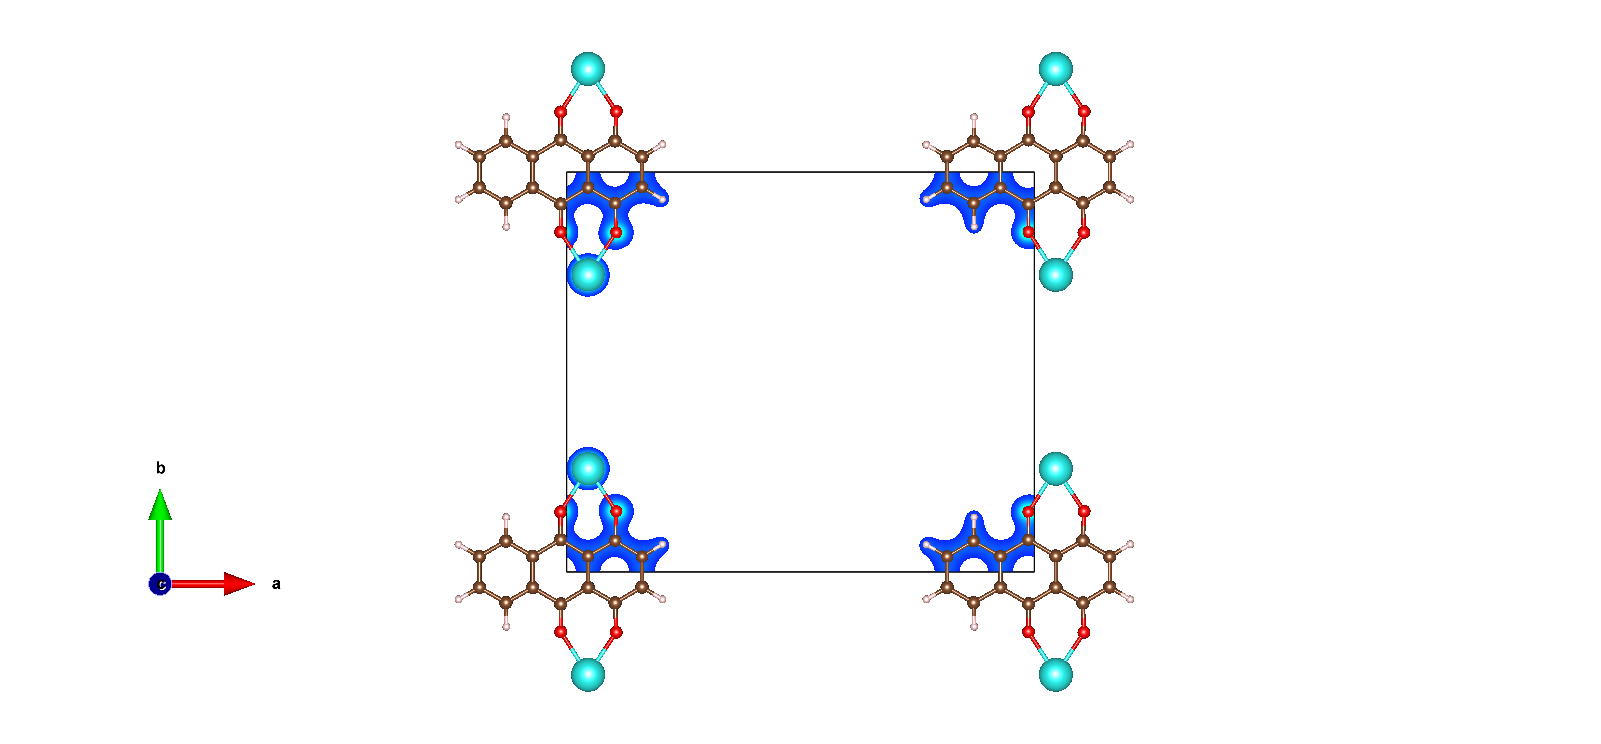
\includegraphics[width = \textwidth]{../fig/Yb_staticbefore_CHGCAR.png}
          \caption{Charge density of Quinizarin with Ytterbium for static VASP calculation. }
          \label{fig:Yb_staticbefore_CHGCAR}
      \end{figure}

      \begin{figure}[H]
          \centering
          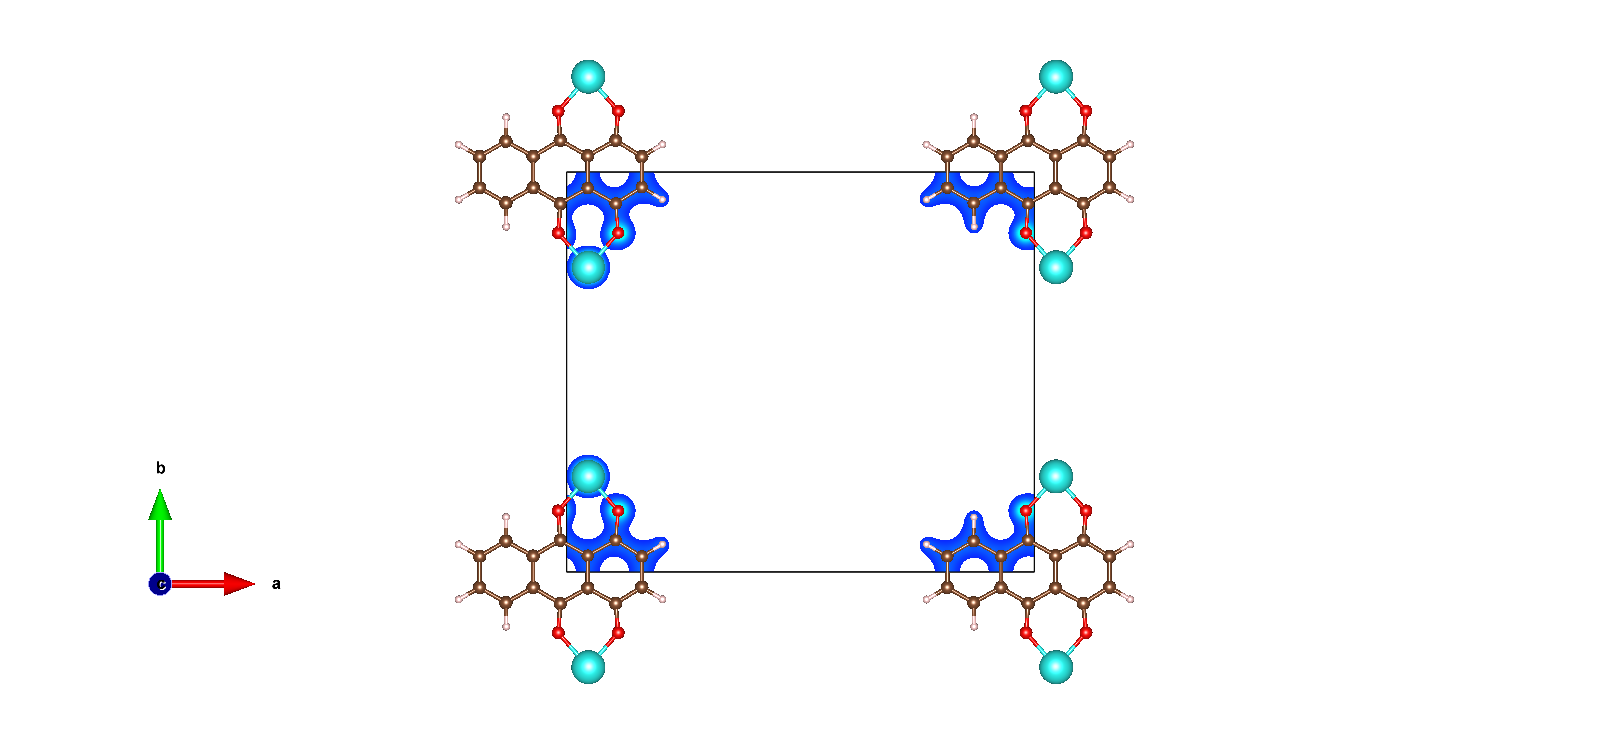
\includegraphics[width = \textwidth]{../fig/Yb_staticafter_CHGCAR.png}
          \caption{Charge density of Quinizarin with Ytterbium for static VASP calculation after relaxed calculation. }
          \label{fig:Yb_staticafter_CHGCAR}
      \end{figure}

      \begin{figure}[H]
        \centering
        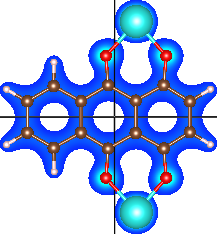
\includegraphics[width = 5cm]{../fig/Yb_staticafter_CHGDENSITY.png}
        \caption{Charge density of a single Quinizarin molecule with Ytterbium for static VASP calculation after relaxed calculation. }
        \label{fig:Yb_staticafter_CHGDENSITY}
      \end{figure}

      \vspace{1cm}

  \subsection{Quinizarin with Neodymium and Thulium}

    We made an attempt to relax the structure with Neodymium and Thulium. This was abandoned, but below, in Figure~(\ref{fig:Nd_relax_CONTCAR}) one can see how one of the attempts at relaxation went. Figure~(\ref{fig:Nd_relax_new_CONTCAR}) shows CONTCAR from a different relaxation attempt. It is worth noting that the unit cells are the same size, but the images were saved with different sizes. \\

      \begin{figure}[H]
        \centering
        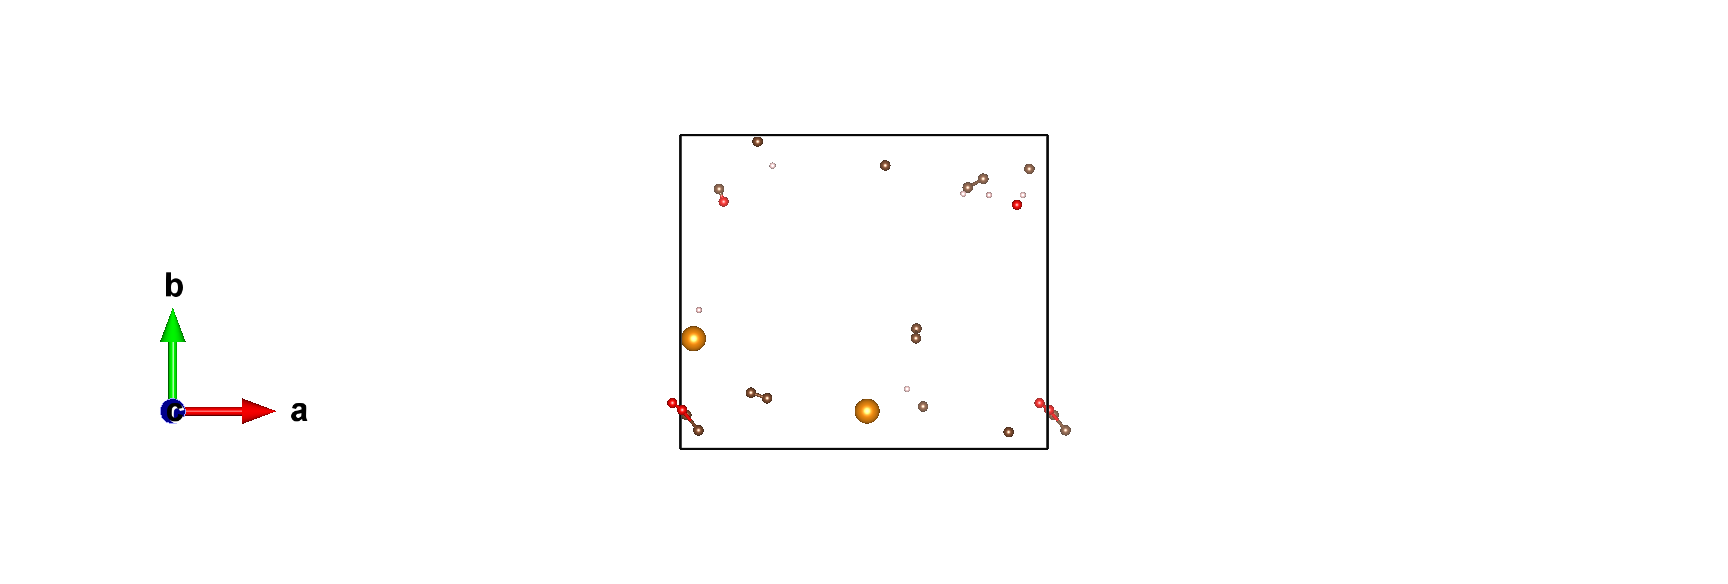
\includegraphics[width = \textwidth]{../fig/Nd_relax_CONTCAR.png}
        \caption{Structure of Quinizarin with Neodymium after relax calculation.}
        \label{fig:Nd_relax_CONTCAR}
      \end{figure}

      \begin{figure}[H]
        \centering
        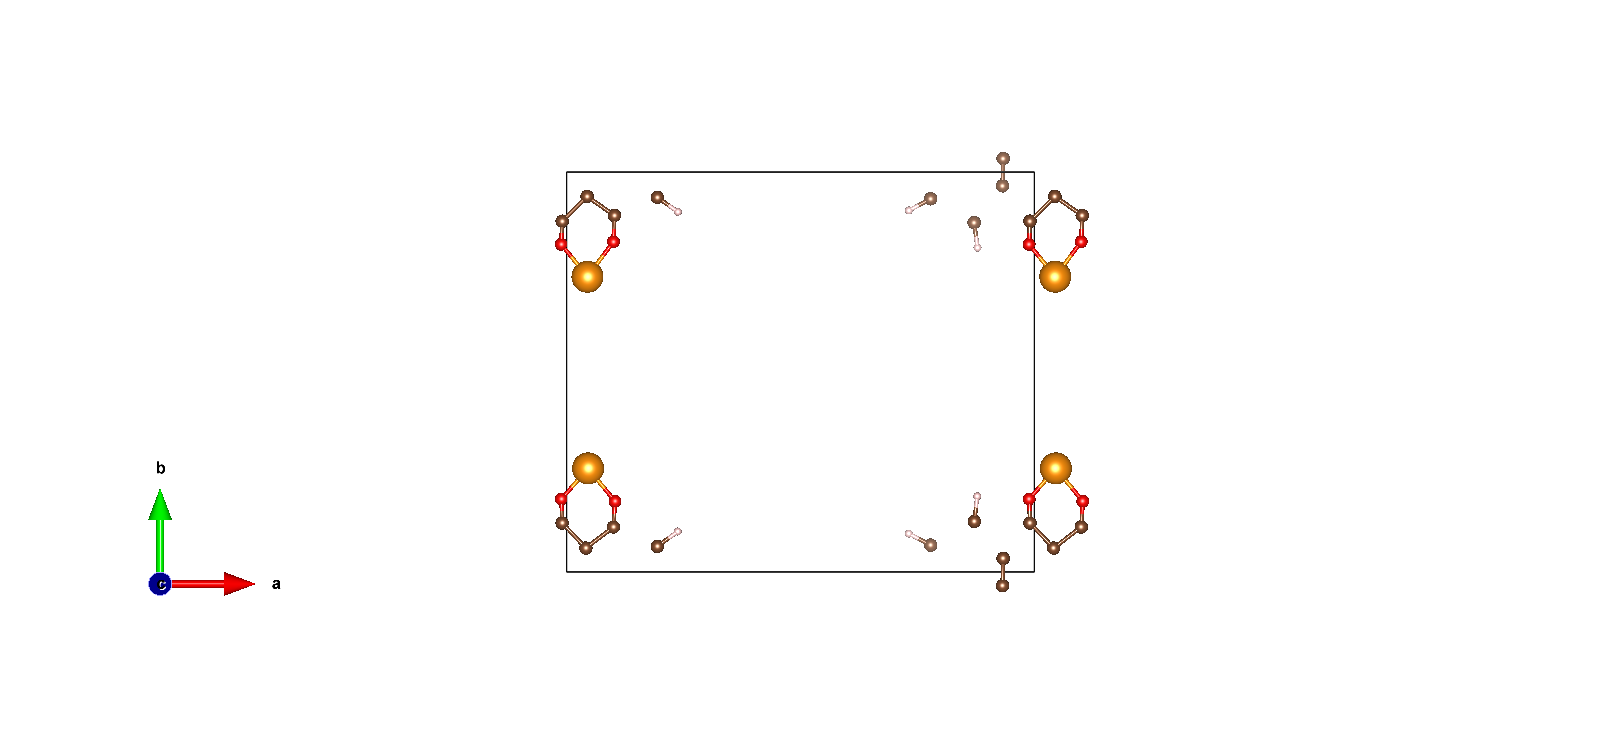
\includegraphics[width = \textwidth]{../fig/Nd_relax_new_CONTCAR.png}
        \caption{Structure of Quinizarin with Neodymium after a different relax calculation.}
        \label{fig:Nd_relax_new_CONTCAR}
      \end{figure}

\vspace{1cm}

\section{Discussion}    \label{sec:Discussion}

  \subsection{Convergence of energy}

    Figure~(\ref{fig:convergence_energy}) shows that the values change quite rapidly and reach a peak around cutoff 500 eV which then lowers and stabilizes near cutoff 800 eV. However, the values differ by a very small amount, which can indicate that one needs a smaller cuttoff energy than 800. Figure~(\ref{fig:convergence_energy_difference}) also indicates this. \\

    From Section~\ref{sec:Convergence} we learned that if the difference in energy is less than 0.003 eV the calculation can be considered converged. The figure shows that ENCUT=450 is below 0.002 eV in difference from ENCUT=500. This shows that ENCUT=450 is safe enough to use. This can seem weird due to it being before a peak and the stabilized total energy is lower, but the values are quite small, and overall should not impact the results in a meaningful way. \\

  \subsection{Convergence of k-points}

    There were fewer data points than with the energy convergence, so it is not as easy to find a pattern as it was with the convergence of energy. For Figure~(\ref{fig:convergence_kpoints}) one can see the energy increases to a peak around 4.0 and 5.0 in k-density, which then decreases at k-density 6.0. Due to the lack of a good pattern we quickly moved on to Figure~(\ref{fig:convergence_kpoints_difference}) which showed even less of a converging pattern. However, already at k-density 1.0 we could see the difference was less than 0.003 eV. Since the difference increased again with 2.0, we wondered if we could use 3.0, but after a few test-calculations with both 1.0 and 3.0 we found the difference was negligible and so we chose to use 1.0. \\

  \subsection{Quinizarin}

    Figure (\ref{fig:basic_staticbefore_CONTCAR}) and Figure (\ref{fig:basic_staticafter_CONTCAR}) compares how the Quinizarin structure differs from before and after a relaxing computation. By examining the figures, there are virtually no difference to be seen. However, Table (\ref{tab:neighborquinizarin}) shows that there actually are a difference. Before relax, the Hydrogen-atoms are at a distance of about 1.75 Å to the double-bonded Oxygen-atoms and at about 0.95 Å to the single-bonded Oxygen-atoms. After relax, the distance has shrunk substantially to the double-bonded Oxygen-atoms to about 1.58 Å. On the contrary has the distances to the single-bonded Oxygen-atoms increased to about 1.03 Å, therefore the change is not as large as for the double-bonded distance. These changes implies a shift of the placement of the Hydrogen-atoms, where they now are closer to the double-bonded Oxygen-atoms than the single-bonded. This shift is explained by that Quinizarin has a resonance structure. A resonance structure implies that an atom has the possibility to shift placement in the structure. In this case for Quinizarin, this means that the Hydrogen-atoms can shift between the double-bonded Oxygen and the single-bonded Oxygen in the alcohol group. Such a shift has another implication, namely that the bond between the Oxygen-atoms and the Carbon-atoms change. For instance if the Hydrogen-atom has a shift further to the left, therefore shorter distance to the double-bonded Oxygen, will the Oxygen-bond to the Carbon have to change to a single-bond to maintain that Oxygen only can share to bonds. The Oxygen in the, now former, alcohol group then has a dangling bond, and forms a double-bond with the Carbon. For this to happen the activation energy has to be enough to break both the single-bond and the double-bond. We do not know the activation energy for Quinizarin, and could not examine when this change in structure forms in this project. However, this is interesting to study for another project. \\

    Table (\ref{tab:TOTENquinizarin}) shows the total energies before and after the relax computation. The total energy after relax is less than before, which is in accordance to that a relaxing computation should make the structure more stable, implying a smaller total energy. The relative energy difference is $-0.015$ eV. \\

    The total density of states shows that there are no half-filled bands, as the fermi level is not inside a band / an orbital. This indicates a lack of unpaired electrons and could tell us that it is diamagnetic. Figure~(\ref{fig:basic_TDOS_2}) also shows that further up there are a lot of orbitals connected which means a broad band that can absorb a lot of different photon energies. This is important for a sensitizer to be able to absort many wavelengths so this is good. LDOS shows that there is not much going on as there are only a few orbitals that Hydrogen use. p and s both contribute about the same amount, which is not to strange as 1s and 1p are fairly close. These figures are almost identical and proves how the upper and lower Hydrogen-atoms have symmetrically equal environments. \\

    In Figure~(\ref{fig:basic_TDOS_2}) we see a band gap from approximately $-0.25$ eV to $1$ eV (scaled to the fermi level). Looking in EIGENVAL we can see a fully occupied band at $-5.31$ eV to a completely empty band at $-3.72$ eV. This corresponds to a band gap of $1.59$ eV, which is not completely in agreement with the figure of DOS, but also not that far off. A band gap of $1.59$ eV corresponds to a semiconductor. This size of band gap means it is quite unlikely for an incoming photon to be re-emitted as phonon vibrations. It will more likely be re-emitted as a photon or, in an up-conversion, be led into the system it self. This is good, and indicates that Quinizarin will not quench any incoming photons. \\

    As for the change in the structure before and after relaxation, the charge density has also not changed much. Figure (\ref{fig:basic_staticbefore_CHGCAR}) and Figure (\ref{fig:basic_staticafter_CHGCAR}) displays the charge density for before relax and after relax, respectively. Table (\ref{tab:neighborquinizarin}) shows that the Hydrogen-atoms move some, but this is not possible to see in the charge density figures either. \\

  \subsection{Quinizarin with Yttrium}  \label{sec:discussionY}

    From relaxing the structure we can see that the atomic distances between the Yttrium and Oxygen atoms decreases. This can both be seen visually in Figure~(\ref{fig:Y_staticbefore_CONTCAR}) and Figure~(\ref{fig:Y_staticafter_CONTCAR}), as well as from the numbers in Table~(\ref{tab:neighborY}). This shows that the initial distances found in ICSD for Ytterbium were not identical for Yttrium. This is good. It was still wise to use 2.32 Å as start distance as the start distance from normal Quinizarin made the molecule explode during ionic relaxation with standard parameters. Another thing to note is how Yttrium is almost in the middle. The initial coordinates also kept Yttrium in the middle, but it is interesting to note how it kept in the middle. It is only 0.01 Å closer to the alcohol-group Oxygen than to the double-bonded Oxygen. This indicates that what used to be double bonds now are single bonds and that both Oxygen's are equally bonded to Yttrium. This is a further step from the resonant structure that was discussed for the normal Quinizarin molecule. \\

    As seen in Table~(\ref{tab:TOTENY}) The energy of Quinizarin with Yttrium after ionic relaxation is lower than before ionic relaxation. This proves that the relaxed structure indeed is relaxed, and shows it being more stable. The relative energy was $-0.109$ eV/atom which shows there was a change, but not a too big one. When it comes to broad-ness in one or more conduction bands this is not as good as normal Quinizarin. There is a band that goes from around $0.5$ eV  to $1.75$ eV, but then there is a gap before a new one pops in around $1.85$ eV. Still, the bond is fairly wide, and will likely absorb a fairly wide spectrum. \\

    The plot over total density of states for Quinizarin with Yttrium shows that there is an orbital at the Fermi level. This means that the orbital is half-full which may indicate that Quinizarin has an unpaired electron spin, making the molecule weakly paramagnetic. One thing to note for the local densities of states is that they both look identical. This shows the mirror symmetry of the molecule. \\

    The band gap was reported to be $0.029$ eV as shown in Table~(\ref{tab:bandgapY}). This is very small and less trustworthy than looking at the density of states. If we observe the density of states there seems to be a bang gap from around 0.25 to 0.75 eV (scaled to Fermi level. Looking in EIGENVAL from the static calculation after relaxation we can see there is a band gap from -3.57 (100\% occupied) to -2.98 (58.1\% occupied). This is a band gap of 0.59 eV, which corresponds fairly well to the gap found in Figure~(\ref{fig:Y_TDOS_2}). This band gap would correspond with a semiconductor, and from gut instinct will likely rather emit the energy absorbed as a photon rather as phonon vibrations. This is good as phonon vibrations will lead to quenching, reducing the efficiency of the up-conversion system. This tells us that a if Quinizarin is embedded in a matrix of YF3 it will likely not quench absorbed photons, and work well as a sensitizer. \\

    Figure (\ref{fig:Y_staticbefore_CHGCAR}) and Figure (\ref{fig:Y_staticafter_CHGCAR}) shows the charge density before relaxation and after relaxation, respectively. As for the basic Quinizarin are there virtually no difference between the two pictures. \\

  \subsection{Quinizarin with Ytterbium}

    Quinizarin with Ytterbium has similar results when comparing how the structure changes before and after relax as Quinizarin with Yttrium, seen in Section \nameref{sec:discussionY}. One similarity is that the Ytterbium-atoms are placed in between of the Oxygen in the alcohol group and the double-bonded Oxygen, this is however mostly for comparison. Another similarity is that after relaxing the structure the Ytterbium moves closer towards the molecule, making the bond length, also called the distance to the double-bonded Oxygen and the single-bonded Oxygen, shorter, while still being maintained in the middle. This can all be seen in Figure (\ref{fig:Yb_staticbefore_CONTCAR}), Figure (\ref{fig:Yb_staticafter_CONTCAR}) and Table (\ref{tab:neighborYb}). In fact, the bond length has approximately the same length as the Quinizarin molecule with Yttrium. However, after relax the bond lengths shrink to both Oxygen-atoms. For both Oxygen-atoms, the distance is cirka 2.32 Å before relax and cirka 2.08 Å after relax. The reasoning behind these changes is therefore the same as for Quinizarin with Yttrium, so the reader is referred to this section. \\

    The total energy of the system changes minimally, but it is more net negative after the relax calculation. Table (\ref{tab:TOTENYb}) shows the total energy before and after the relaxation. The relative energy is a $-0.013$ eV difference. Quinizarin with Ytterbium is therefore more stable after relaxation. \\

    Figure~(\ref{fig:Yb_TDOS_2}) shows the density of states for Quinizarin with Ytterbium. Immediately we see that the Fermi level is inside a bond which again can indicate unpaired electrons and the molecule being weakly paramagnetic. After around $1.8$ eV there seems to be a very wide band going all the way up to and past $3$ eV. A small dip around $2.5$ eV, but not a complete gap. This is incredibly good as it means the molecule might absorb photons for the whole spectrum of available light. The LDOS figures show that d-orbitals contribute the most, while s-orbitals the least, with p-orbitals between those two. There is a massive f-orbital right near the Fermi level. These are also identical between the upper and lower Ytterbium atoms. \\

    There seems to be a band gap from around $0.33$ eV to $1.2$ eV. In EIGENVAL we see that there is a fully occupied band at $-3.05$ eV, and the next band is at $2.72$ eV and is $67\%$ occupied. This corresponds to a band gap of $0.33$ eV. This is quite low and would correspond to a metallic semiconductor in gap size. This is fairly low and could mean that optical phonon vibrations are possible. This could indicate that though Quinizarin with Yb works very well as a sensitizer it could also participate in quenching. This means that the excited electron has to be moved quickly, in order to avoid de-excitation and loss in efficiency. \\

    The charge density for Quinizarin with Ytterbium is shown in Figure (\ref{fig:Yb_staticbefore_CHGCAR}) and Figure (\ref{fig:Yb_staticafter_CHGCAR}), where they show before relaxation and after relaxation, respectively. Similarly with the other Quinizarin-structures are there no visible changes between these two pictures. This is because the atoms themselves does not change electronegativity before and after a relaxation. \\

  \subsection{Quinizarin with Neodymium and Thulium}

    We attempted to perform relaxation and evaluation of Quinizarin with Neodymium and Thulium as well. Initially we attempted with the relaxed Hydrogen-system as POSCAR for these atoms, but the distance was way to low. This resulted in an explosion of the molecule a lack of relaxation. We then tried to relax with more electronic steps, but this did not help. This was also the case for Y and Yb initially. After using around 2.3 Å as distance (after looking at various solid structures on ICSD) we managed to get a relaxed structure for Y and Yb. However, this was not the case for Nd and Tm. We then tried to increase the amount of electronic steps, NELM, to 300, without success. We cross-checked some Nd-structures on ICSD, but 2.3 Å seemed reasonable to use. After a final attempt with IBRION=2 and POTIM=0.2 we hoped for a better result. This was not the case, as after 3 hours it still had not converged. We weighed our options of either increasing the maximum time, or to stop trying with Nd and Tm. After a talk with our supervisors we decided to only report for Y and Yb. \\

  \subsection{Total comparison}

    First of all we can see that the Hydrogen-Oxygen distance is much lower than the Yttrium-Oxygen distances and the Ytterbium-Oxygen distances. This makes a lot of sense as Hydrogen is incredibly small in comparison. Beyond this we see that Yttrium-Oxygen has a smaller distance than Ytterbium-Oxygen. This is likely due to Ytterbium's large size from f-orbitals. \\

    Quinizarin had a total energy per atom of $-7.034$ eV, which gives Quinizarin with Yttrium a relative energy of $0.242$ eV. This shows that normal Quinizarin is more stable. However, exchanging Hydrogen with Yttrium should not be to energy-intensive. Quinizarin with Ytterbium has a relative energy to normal Quinizarin of $-0.152$ eV, and $-0.394$ eV versus Quinizarin with Yttrium. This shows that even though Ytterbium is a large atom that can seem unwieldy, it is quite stable in Quinizarin. This can mean the an up-conversion system in a YbF3-matrix with Quinizarin as a sensitizer is quite stable. At the same time, this low relative energy could be attributed to the fact that the initial POSCAR was made with Yb in mind, meaning that it is easier to relax the structure with Yb than with Y. However, a quick check of vaspout for both static calculations after ionic relaxation show that the max force of Quinizarin with Yb is $0.1660$, wheras Quinizarin with Y has a max force of $0.0354$. This shows that they are both very relaxed, and that the low relative energy of Ytterbium is in fact trustworthy. \\

    Comparing the densities of states for the different molecules we observe that normal Quinizarin is quite boring when it comes to LDOS due to Hydrogen not having a lot of orbitals to contribute with. There is a wide band around $5$ eV which can be utilized for sensitization. Here Quinizarin with Yttrium has a narrow band for the same use-case. Ytterbium has an extremely wide band that functions well for sensitizatin. LDOS shows that more action for Yttrium and Ytterbium, with d-orbitals participating a lot. For Ytterbium the f-orbital is very high, and but is below the Fermi level so is not as interesting as its d-orbitals above the Fermi level. \\

    Normal Quinizarin shows a band gap of $1.59$ eV, whilst Quinizarin with Yttrium shows a band gap of $0.59$ eV, and Quinizarin with Ytterbium an even lower gap with $0.33$ eV. This shows how changing the atom on the Oxygen bridge impacts the band gap in major way. The lower band gaps indicates a higher risk of optical phonon vibrations rather than an emitted photon, but as long as the excited electron gets to move away quickly this issue should be minimized. The smaller size of band gaps also show that they can absorb photons with lower energy, but this is only useful if they can be transferred in the up-conversion system and utilized for the actual up-conversion. \\

    Comparing the charge density for before and after relaxation for the three Quinizarin structures proved to be of little interest, however the comparison between the structures illustrates the difference in the substitutional atoms. Figure (\ref{fig:basic_staticafter_CHGDENSITY}), Figure (\ref{fig:Y_staticafter_CHGDENSITY}) and Figure (\ref{fig:Yb_staticafter_CHGDENSITY}) shows the charge density for molecules of Quinizarin, Quinizarin with Yttrium, and Quinizarin with Ytterbium, respectively. These pictures are after a relax computation. The booklet \textit{Gyldendals tabeller og formler i kjemi : kjemi 1 og kjemi 2} has an overview of the electronegativities for multiple atoms. This says that the electronegativity of Oxygen is 3.5, for Hydrogen is 2.1, for Carbon is 2.5, for Yttrium is 1.2, and for Yb is 1.1 \cite{kjemibok}. The charge density for Quinizarin and Quinizarin with Yttrium is mostly in accordance with this. The Oxygen-atoms are the most electronegative, so they should have the highest charge density, which is correct from the images. However, Quinizarin with Ytterbium is not in accordance with the electronegativity of the atoms. The Ytterbium-atoms are very large in comparison to the other atoms, so it is difficult to see what charge density they have. The Oxygen-atoms and the Carbon-atoms should nonetheless have a much higher charge density than what is depicted in the figures. In these figures they have a very dark blue color, which means very small charge density. Therefore, we theorize that the Ytterbium-atoms have a very high charge density, which we cannot see. This is however not at all in accordance with the electronegativities. Ytterbium has the lowest electronegativity of all the atoms listed above, and should not have a high charge density. We concluded from this that something must have gone wrong with the computation of the charge density, which we do not know what is. \\

\vspace{1cm}

\section{Conclusion}    \label{sec:Conclusion}

  After gaining insight into performing calculations with VASP, we moved on to performing convergence tests. This showed that a cutoff energy of $450$ eV was sufficient, and a k-density of $1.0$ worked well. There were some issues with relaxing the structures of Yttrium and Ytterbium, but these were resolved after searching up atomic distance data for various bulk compounds. Of all three systems, Ytterbium seemed most stabile in energy. This was surprising, but not unwelcome, as Ytterbium also proved to have a wide band gap ideal for absorbing a wide spectrum of photons. Yttrium had a narrower band gap, which could prove unhelpful. When band gaps were looked into Yttriums gap of $0.59$ seemed large enough to avoid de-exications by optical phonon vibrations, but this was more worrying for Ytterbium which showed a band gap of $0.33$ eV. However, as long as photons that create these phonon vibrations are avoided, and the excited electrons are moved fast enough away this should be a small issue with efficiency of the up-conversion system. Charge density seemed quite of for Ytterbium which also can be a problem. However, in total, Ytterbium seems like an atom with so many positives that it is at least worth testing the up-conversion system with it, before exploring other options. Yttrium will be interesting to investigate as a different option.

%--------------------- References --------------------------------------------
\vspace{1cm}

\section{References} \label{sec:References}

    \begin{thebibliography}{}

    \bibitem{kjemibok}
    Bjørn-Gunnar Steen, 2009, \textit{Gyldendals tabeller og formler i kjemi : kjemi 1 og kjemi 2}, Gyldendal undervisning.

    \bibitem{github}
    Erlend Tiberg North, Alexandra Jahr Kolstad, 2020, \url{https://github.com/alexanjk/FYS-MENA4111-projectH20}, \textit{Github repository with figures and python-scripts for graph-plotting and LaTeX files}, University of Oslo.

    \bibitem{saga}
    Erlend Tiberg North, Alexandra Jahr Kolstad, 2020, \textit{Saga directory with all runs and raw data, /cluster/projects/nn9989k/quinizarin\_AJK\_ETN/}, University of Oslo \& Sigma2.

    \bibitem{icsd}
     FIZ Karlsruhe, 2020, \url{https://icsd-fiz-karlsruhe-de.ezproxy.uio.no/display/list.xhtml}, ICSD.


    \end{thebibliography}


%------------------ Appendix ------------------------------------

\appendix

\section*{Appendix} \label{sec:Appendix}

\section{Quinizarin-pictures}

  \begin{figure}[H]
      \centering
      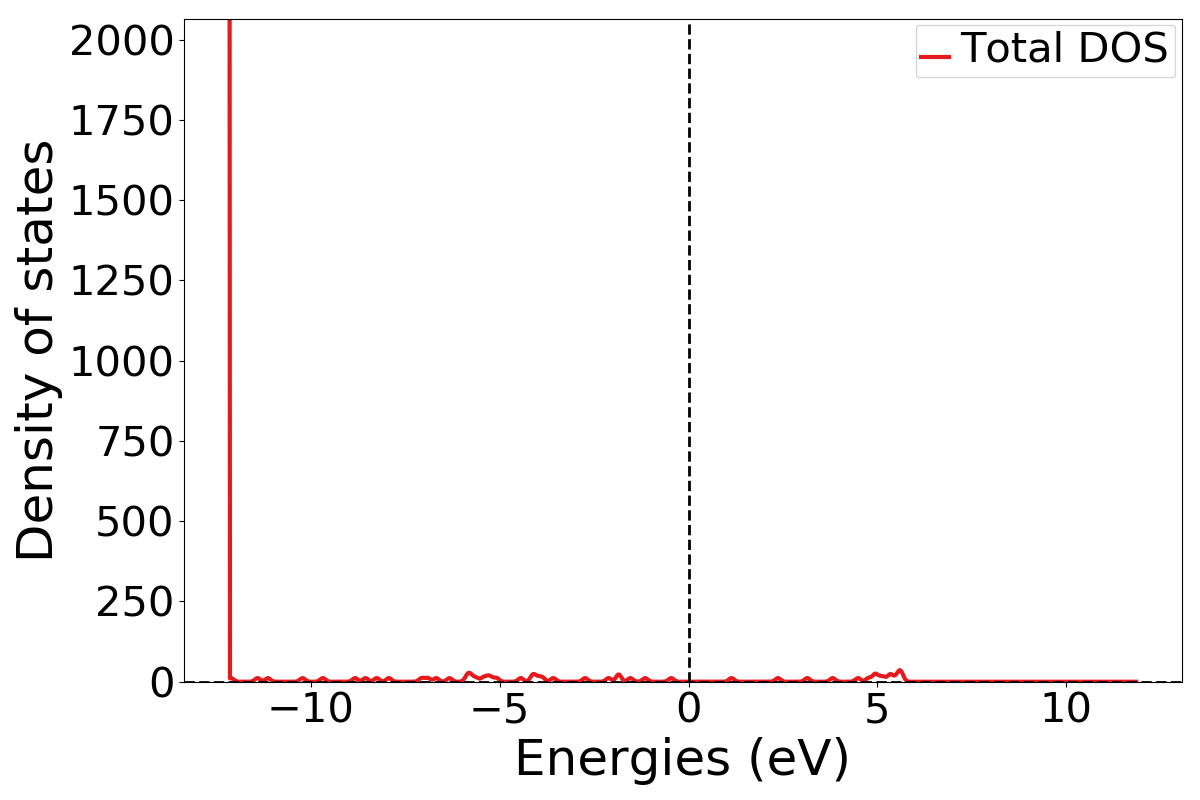
\includegraphics[width = 11cm]{../fig/basic_TDOS_1.png}
      \caption{Plot of total DOS for Quinizarin. }
      \label{fig:basic_TDOS_1}
  \end{figure}

  \begin{figure}[H]
      \centering
      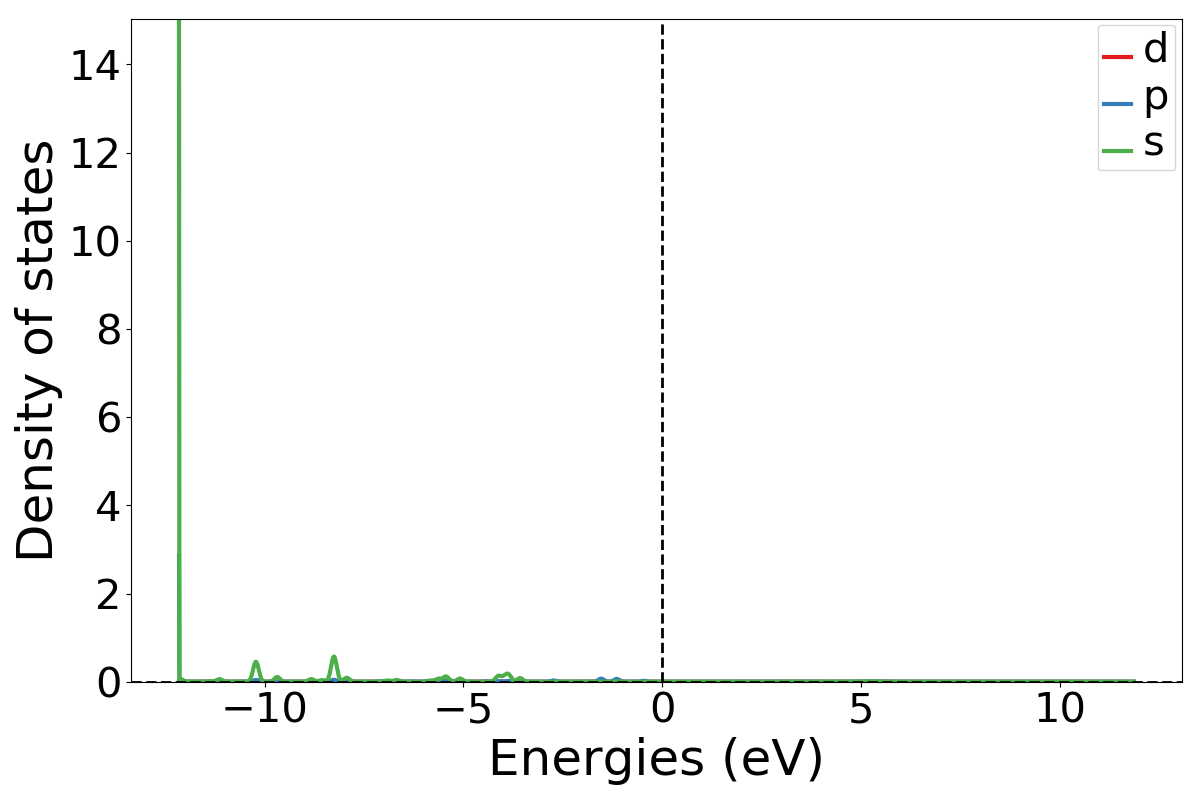
\includegraphics[width = 11cm]{../fig/basic_LDOS25_1.png}
      \caption{Plot of local DOS for atom number 25(H in alcohol-group) for Quinizarin.}
      \label{fig:basic_LDOS25_1}
  \end{figure}

  \begin{figure}[H]
      \centering
      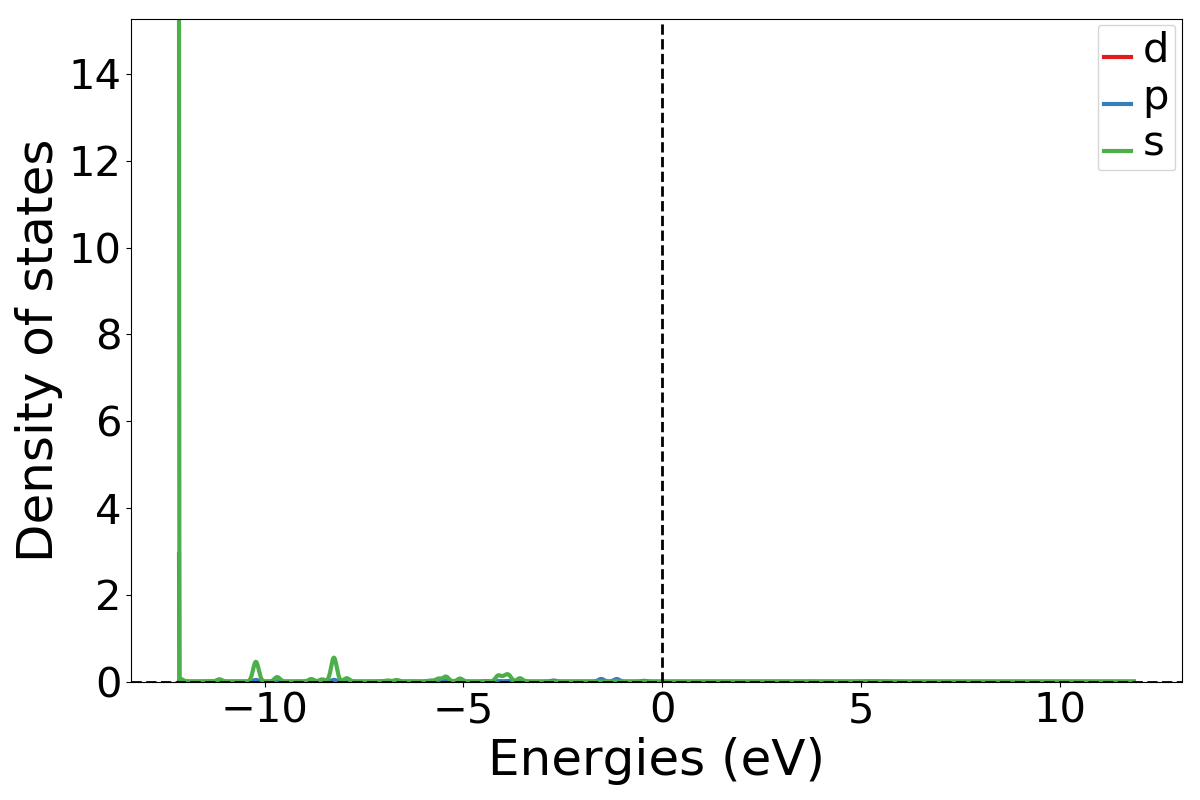
\includegraphics[width = 11cm]{../fig/basic_LDOS26_1.png}
      \caption{Plot of local DOS for atom number 26(H in alcohol-group) for Quinizarin. }
      \label{fig:basic_LDOS26_1}
  \end{figure}

\vspace{1cm}

\section{Y-pictures}

  \begin{figure}[H]
      \centering
      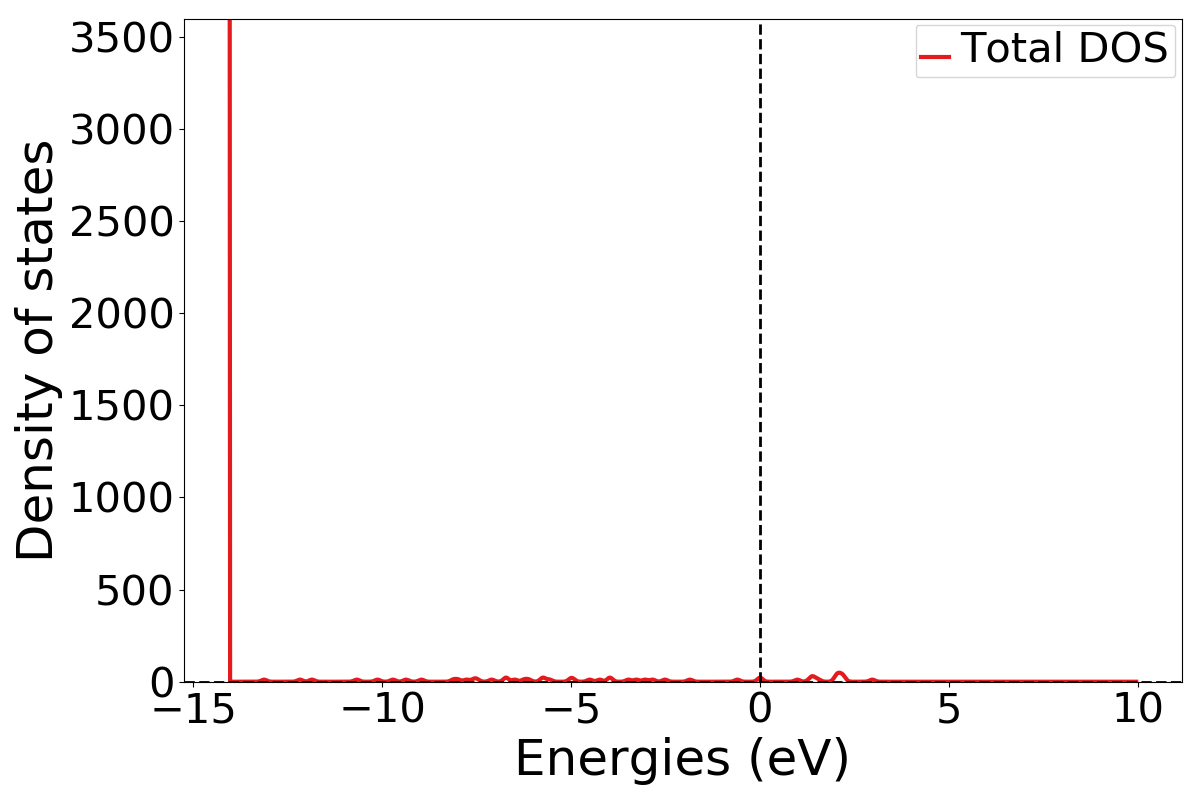
\includegraphics[width = 11cm]{../fig/Y_TDOS_1.png}
      \caption{Plot of total DOS for Quinizarin with Yttrium. }
      \label{fig:Y_TDOS_1}
  \end{figure}

  \begin{figure}[H]
      \centering
      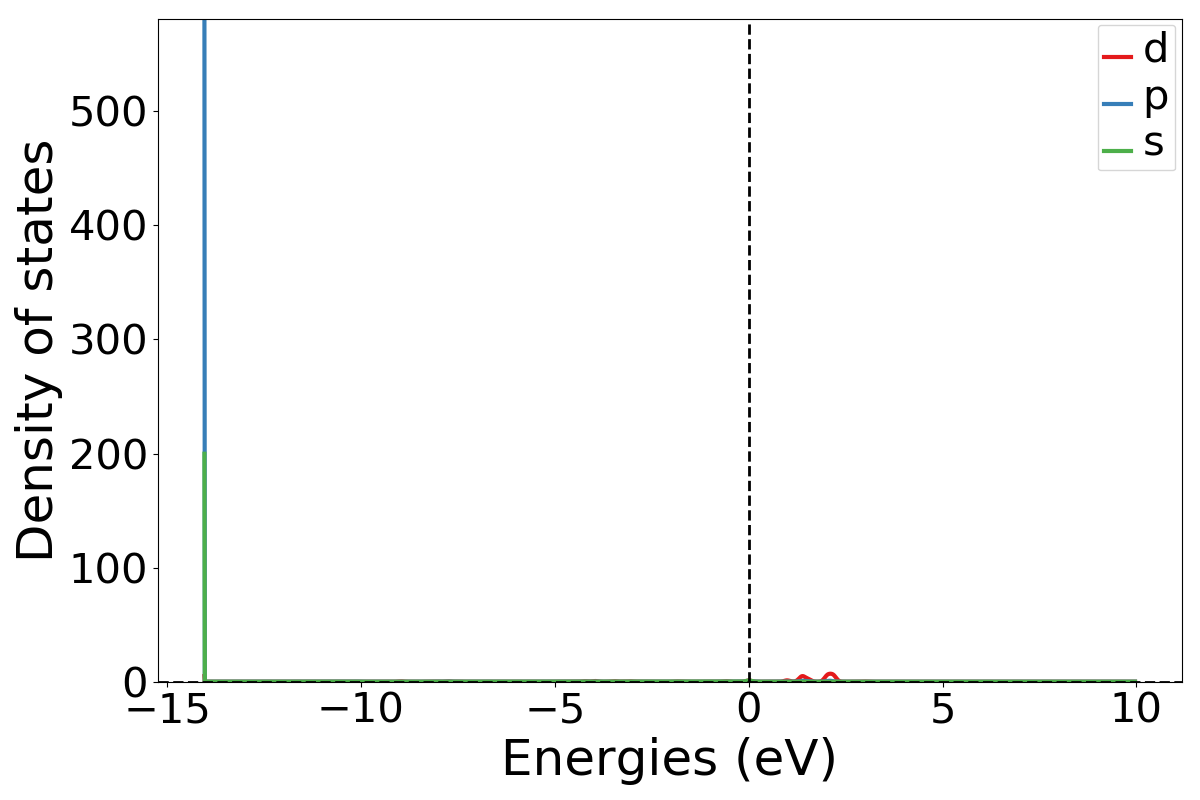
\includegraphics[width = 11cm]{../fig/Y_LDOS25_1.png}
      \caption{Plot of local DOS of atom number 25(Y in lower alcohol-group) for Quinizarin with Yttrium. }
      \label{fig:Y_LDOS25_1}
  \end{figure}

  \begin{figure}[H]
      \centering
      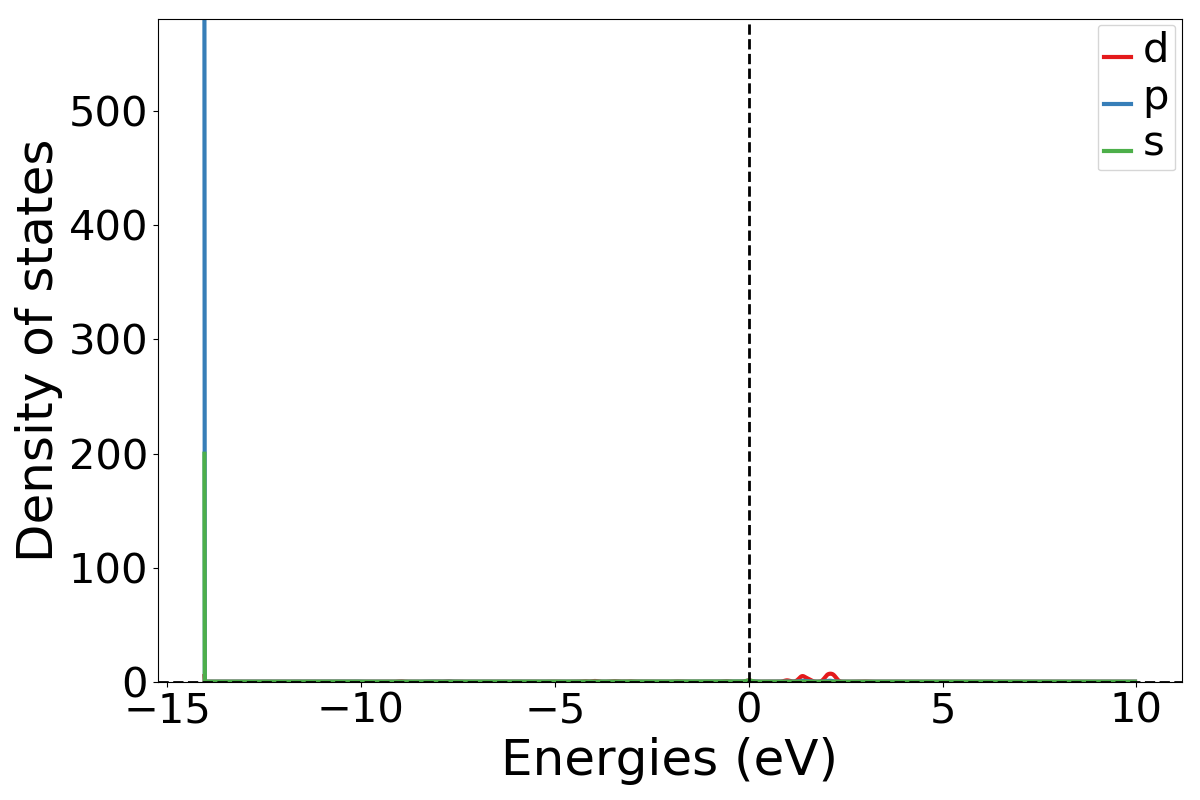
\includegraphics[width = 11cm]{../fig/Y_LDOS26_1.png}
      \caption{Plot of local DOS of atom number 26(Y in upper alcohol-group) for Quinizarin with Yttrium. }
      \label{fig:Y_LDOS26_1}
  \end{figure}

\vspace{1cm}

\section{Yb-pictures}

  \begin{figure}[H]
      \centering
      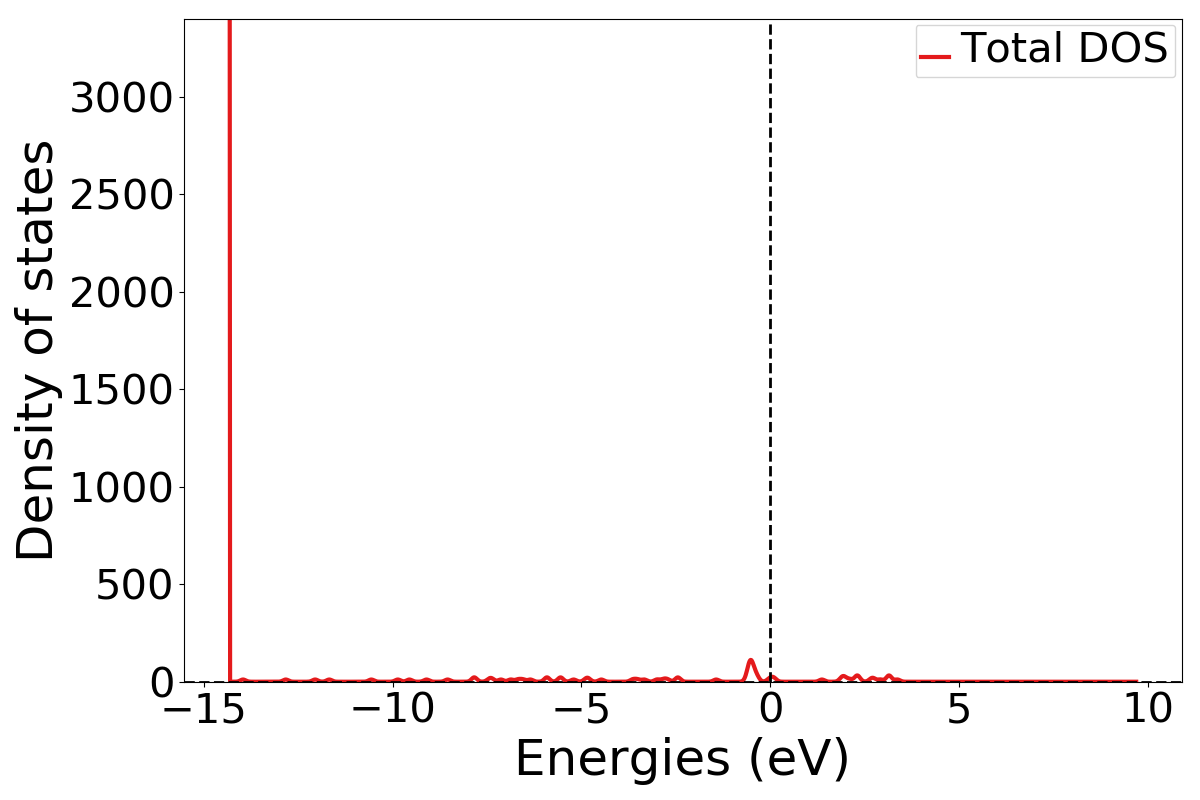
\includegraphics[width = 11cm]{../fig/Yb_TDOS_1.png}
      \caption{Plot of total DOS for Ytterbium. }
      \label{fig:Yb_TDOS_1}
  \end{figure}

  \begin{figure}[H]
      \centering
      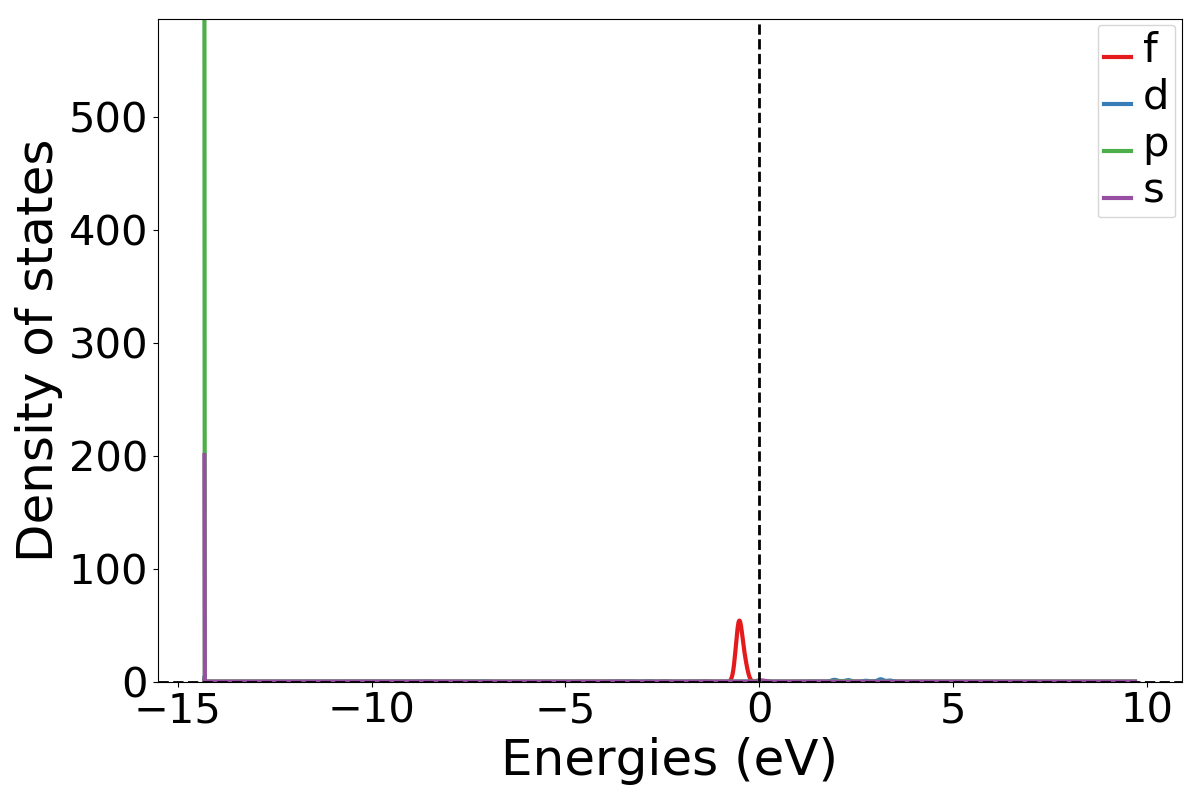
\includegraphics[width = 11cm]{../fig/Yb_LDOS25_1.png}
      \caption{Plot of local DOS of atom number 25(Yb in lower alcohol-group) for Quinizarin with Ytterbium. }
      \label{fig:Yb_LDOS25_1}
  \end{figure}

  \begin{figure}[H]
      \centering
      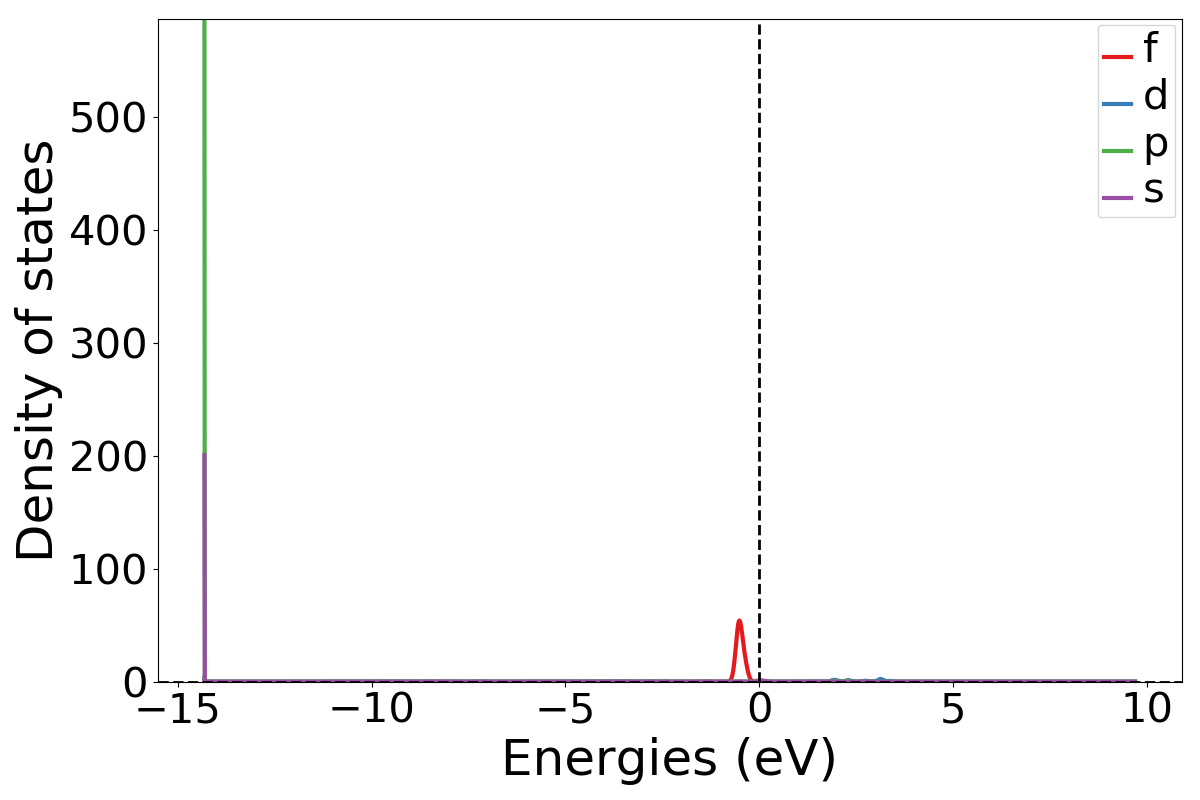
\includegraphics[width = 11cm]{../fig/Yb_LDOS26_1.png}
      \caption{Plot of local DOS of atom number 26(Yb in upper alcohol-group) for Quinizarin with Ytterbium. }
      \label{fig:Yb_LDOS26_1}
  \end{figure}

%---------------- Slutten av dokumentet ---------------------------------------

%\end{multicols}

\end{document}
